%Version 3.1 December 2024
% See section 11 of the User Manual for version history
%
%%%%%%%%%%%%%%%%%%%%%%%%%%%%%%%%%%%%%%%%%%%%%%%%%%%%%%%%%%%%%%%%%%%%%%
%%                                                                 %%
%% Please do not use \input{...} to include other tex files.       %%
%% Submit your LaTeX manuscript as one .tex document.              %%
%%                                                                 %%
%% All additional figures and files should be attached             %%
%% separately and not embedded in the \TeX\ document itself.       %%
%%                                                                 %%
%%%%%%%%%%%%%%%%%%%%%%%%%%%%%%%%%%%%%%%%%%%%%%%%%%%%%%%%%%%%%%%%%%%%%

%%\documentclass[referee,sn-basic]{sn-jnl}% referee option is meant for double line spacing

%%=======================================================%%
%% to print line numbers in the margin use lineno option %%
%%=======================================================%%

%%\documentclass[lineno,pdflatex,sn-basic]{sn-jnl}% Basic Springer Nature Reference Style/Chemistry Reference Style

%%=========================================================================================%%
%% the documentclass is set to pdflatex as default. You can delete it if not appropriate.  %%
%%=========================================================================================%%

%%\documentclass[sn-basic]{sn-jnl}% Basic Springer Nature Reference Style/Chemistry Reference Style

%%Note: the following reference styles support Namedate and Numbered referencing. By default the style follows the most common style. To switch between the options you can add or remove “Numbered” in the optional parenthesis. 
%%The option is available for: sn-basic.bst, sn-chicago.bst%  
 
%%\documentclass[pdflatex,sn-nature]{sn-jnl}% Style for submissions to Nature Portfolio journals
%%\documentclass[pdflatex,sn-basic]{sn-jnl}% Basic Springer Nature Reference Style/Chemistry Reference Style
\documentclass[pdflatex,sn-mathphys-num]{sn-jnl}% Math and Physical Sciences Numbered Reference Style
%%\documentclass[pdflatex,sn-mathphys-ay]{sn-jnl}% Math and Physical Sciences Author Year Reference Style
%%\documentclass[pdflatex,sn-aps]{sn-jnl}% American Physical Society (APS) Reference Style
%%\documentclass[pdflatex,sn-vancouver-num]{sn-jnl}% Vancouver Numbered Reference Style
%%\documentclass[pdflatex,sn-vancouver-ay]{sn-jnl}% Vancouver Author Year Reference Style
%%\documentclass[pdflatex,sn-apa]{sn-jnl}% APA Reference Style
%%\documentclass[pdflatex,sn-chicago]{sn-jnl}% Chicago-based Humanities Reference Style

%%%% Standard Packages
%%<additional latex packages if required can be included here>

\usepackage{graphicx}%
\usepackage{multirow}%
\usepackage{amsmath,amssymb,amsfonts}%
\usepackage{amsthm}%
\usepackage{mathrsfs}%
\usepackage[title]{appendix}%
\usepackage{xcolor}%
\usepackage{textcomp}%
\usepackage{manyfoot}%
\usepackage{booktabs}%
\usepackage{algorithm}%
\usepackage{algorithmicx}%
\usepackage{algpseudocode}%
\usepackage{listings}%
\usepackage{lmodern}%
%%%%

%%%%%=============================================================================%%%%
%%%%  Remarks: This template is provided to aid authors with the preparation
%%%%  of original research articles intended for submission to journals published 
%%%%  by Springer Nature. The guidance has been prepared in partnership with 
%%%%  production teams to conform to Springer Nature technical requirements. 
%%%%  Editorial and presentation requirements differ among journal portfolios and 
%%%%  research disciplines. You may find sections in this template are irrelevant 
%%%%  to your work and are empowered to omit any such section if allowed by the 
%%%%  journal you intend to submit to. The submission guidelines and policies 
%%%%  of the journal take precedence. A detailed User Manual is available in the 
%%%%  template package for technical guidance.
%%%%%=============================================================================%%%%

%% as per the requirement new theorem styles can be included as shown below
\theoremstyle{thmstyleone}%
\newtheorem{theorem}{Theorem}%  meant for continuous numbers
%%\newtheorem{theorem}{Theorem}[section]% meant for sectionwise numbers
%% optional argument [theorem] produces theorem numbering sequence instead of independent numbers for Proposition
\newtheorem{proposition}[theorem]{Proposition}% 
%%\newtheorem{proposition}{Proposition}% to get separate numbers for theorem and proposition etc.

\theoremstyle{thmstyletwo}%
\newtheorem{example}{Example}%
\newtheorem{remark}{Remark}%

\theoremstyle{thmstylethree}%
\newtheorem{definition}{Definition}%

\raggedbottom
%%\unnumbered% uncomment this for unnumbered level heads

\begin{document}

\title[Article Title]{Thermodynamic-limit quantum many-body inference with discrete diffusion}

%%=============================================================%%
%% GivenName	-> \fnm{Joergen W.}
%% Particle	-> \spfx{van der} -> surname prefix
%% FamilyName	-> \sur{Ploeg}
%% Suffix	-> \sfx{IV}
%% \author*[1,2]{\fnm{Joergen W.} \spfx{van der} \sur{Ploeg} 
%%  \sfx{IV}}\email{iauthor@gmail.com}
%%=============================================================%%

\author*[1,2]{\fnm{First} \sur{Author}}\email{iauthor@gmail.com}

\author[2,3]{\fnm{Second} \sur{Author}}\email{iiauthor@gmail.com}
\equalcont{These authors contributed equally to this work.}

\author[1,2]{\fnm{Third} \sur{Author}}\email{iiiauthor@gmail.com}
\equalcont{These authors contributed equally to this work.}

\affil*[1]{\orgdiv{Department}, \orgname{Organization}, \orgaddress{\street{Street}, \city{City}, \postcode{100190}, \state{State}, \country{Country}}}

\affil[2]{\orgdiv{Department}, \orgname{Organization}, \orgaddress{\street{Street}, \city{City}, \postcode{10587}, \state{State}, \country{Country}}}

\affil[3]{\orgdiv{Department}, \orgname{Organization}, \orgaddress{\street{Street}, \city{City}, \postcode{610101}, \state{State}, \country{Country}}}

%%==================================%%
%% Sample for unstructured abstract %%
%%==================================%%

\abstract{Quantum many-body systems exhibit emergent phenomena that often become fully characterized only in the thermodynamic limit, yet direct measurement and simulation at large system sizes remain prohibitively challenging. Here we introduce Diffushadow, a discrete diffusion framework for scalable quantum measurement generation from classical-shadow data. Diffushadow represents randomized Pauli measurements as interleaved token sequences and employs full-attention iterative denoising to model globally correlated measurement configurations without imposing an autoregressive ordering. Trained only on small-system measurement data, Diffushadow generates physically consistent measurements at both training sizes and larger unseen system sizes across representative one-dimensional spin-chain Hamiltonians, including the transverse-field Ising model, the frustrated \(J_1\)-\(J_2\) model, and the ANNNI model. Building on this cross-scale generation capability, we develop a recursive scale extrapolation procedure that progressively expands the accessible system size and enables finite-size scaling toward the thermodynamic limit. Using generated measurements, Diffushadow estimates thermodynamic-limit spin-spin correlation profiles in the transverse-field Ising model, with additional validation on frustrated and competing-interaction spin chains. Attention analysis further reveals spatial attention patterns aligned with physical correlation structures, providing a mechanistic perspective on the learned transferable measurement representations. Overall, Diffushadow demonstrates that generative modeling of small-system quantum measurements can support scalable inference of many-body physics in the thermodynamic limit.
}


%%================================%%
%% Sample for structured abstract %%
%%================================%%

% \abstract{\textbf{Purpose:} The abstract serves both as a general introduction to the topic and as a brief, non-technical summary of the main results and their implications. The abstract must not include subheadings (unless expressly permitted in the journal's Instructions to Authors), equations or citations. As a guide the abstract should not exceed 200 words. Most journals do not set a hard limit however authors are advised to check the author instructions for the journal they are submitting to.
% 
% \textbf{Methods:} The abstract serves both as a general introduction to the topic and as a brief, non-technical summary of the main results and their implications. The abstract must not include subheadings (unless expressly permitted in the journal's Instructions to Authors), equations or citations. As a guide the abstract should not exceed 200 words. Most journals do not set a hard limit however authors are advised to check the author instructions for the journal they are submitting to.
% 
% \textbf{Results:} The abstract serves both as a general introduction to the topic and as a brief, non-technical summary of the main results and their implications. The abstract must not include subheadings (unless expressly permitted in the journal's Instructions to Authors), equations or citations. As a guide the abstract should not exceed 200 words. Most journals do not set a hard limit however authors are advised to check the author instructions for the journal they are submitting to.
% 
% \textbf{Conclusion:} The abstract serves both as a general introduction to the topic and as a brief, non-technical summary of the main results and their implications. The abstract must not include subheadings (unless expressly permitted in the journal's Instructions to Authors), equations or citations. As a guide the abstract should not exceed 200 words. Most journals do not set a hard limit however authors are advised to check the author instructions for the journal they are submitting to.}

\keywords{quantum many-body systems, discrete diffusion models, thermodynamic-limit inference, finite-size scaling, mechanistic interpretability}

%%\pacs[JEL Classification]{D8, H51}

%%\pacs[MSC Classification]{35A01, 65L10, 65L12, 65L20, 65L70}

\maketitle

\section{Introduction}\label{sec1}

Quantum many-body systems exhibit rich emergent phenomena arising from collective quantum interactions \cite{tokura2017emergent, bruus2004many}. Phenomena such as quantum phase transitions, magnetism, superconductivity, and topological order are central to condensed matter physics, quantum materials, and quantum information science \cite{defenu2024out}. Understanding these phenomena is essential, yet many fundamental properties of quantum matter only fully emerge in the thermodynamic limit, where the number of interacting particles becomes extremely large \cite{sachdev1999quantum}.
However, characterizing quantum many-body systems at thermodynamic scales remains fundamentally challenging because the dimension of the Hilbert space grows exponentially with system size \cite{eisert2010colloquium}. Although recent advances in programmable quantum simulators and quantum computers have enabled the preparation of increasingly complex quantum states \cite{bourgund2025formation, king2025beyond}, obtaining and analyzing large-scale quantum measurements remain prohibitively expensive in physical experiments, while classical numerical simulations rapidly become computationally intractable as system size increases. As a result, developing scalable approaches capable of inferring thermodynamic-scale quantum behavior from limited experimentally accessible measurements remains a fundamental open challenge in quantum many-body physics.
% However, large-scale quantum systems pose substantial difficulties for researchers at present. Due to the exponential growth of the state space with the system size, describing and characterizing large-scale quantum systems becomes extremely difficult and even infeasible for classical computers. Although advanced methods like classical shadow tomography offer more efficient ways to estimate properties, obtaining the required experimental data still necessitates a significant amount of physical experiments or computational resources. As a result, developing scalable approaches capable of inferring thermodynamic-scale quantum behavior from limited accessible measurements remains a fundamental open challenge in quantum many-body physics.


In recent years, machine learning has emerged as a promising approach for addressing this challenge by enabling scalable, data-driven characterization of quantum systems \cite{carleo2019machine, carleo2017solving}. Machine learning, particularly generative models, has demonstrated the capacity to effectively learn physical properties and representations of quantum many-body systems directly from experimentally accessible measurements \cite{carrasquilla2017machine, liu2018differentiable}. Methods employing these techniques have been successfully applied to tasks including quantum property prediction \cite{schutt2017schnet, wanner2024predicting, yao2024shadowgpt}, phase classification \cite{cho2024machine}, quantum state reconstruction \cite{torlai2018neural, carrasquilla2019reconstructing}, and surrogate modeling of quantum systems \cite{pfau2020ab}. 



However, many learning-based approaches to quantum state modeling, tomography, and measurement generation are formulated and evaluated at prescribed system sizes, where the dimensionality of the measurement configuration is fixed during training and inference \cite{chinzei2025learning, torlai2018neural}. Cross-scale generalization toward substantially larger systems is therefore not typically the central objective of these frameworks, leaving their applicability limited in scenarios where direct large-scale training data are unavailable \cite{cho2024machine}. This limitation is especially critical because many essential properties of quantum matter, including long-range correlations and critical phenomena, only fully emerge at sufficiently large scales and in the thermodynamic limit \cite{fisher1972scaling}. This raises the fundamental question of whether scalable quantum behavior can be inferred from measurements available only at small system sizes. In particular, it remains unclear whether generative models can learn transferable quantum measurement structures that persist across scales and support inference toward the thermodynamic limit.
% However, most existing methods remain restricted to fixed system sizes, where training and inference are performed within the same accessible scale regime \cite{chinzei2025learning}. As a result, their applicability to larger quantum systems remains limited, particularly in scenarios where direct large-scale training data are unavailable \cite{cho2024machine}. This limitation is especially critical because many essential properties of quantum matter, including long-range correlations and critical phenomena, only fully emerge at sufficiently large scales and in the thermodynamic limit. This raises the fundamental question of whether scalable quantum behavior can be inferred from measurements available only at small system sizes. In particular, it remains unclear whether generative models can learn transferable quantum measurement structures that persist across scales and support inference toward the thermodynamic limit.
Autoregressive architectures have been widely used for discrete sequence modeling in domains such as language, images, and audio~\cite{vaswani2017attention,van2016pixel,van2016wavenet}, and have recently been adopted for quantum many-body modeling and randomized-measurement generation~\cite{sharir2020deep,hibat2020recurrent,yao2024shadowgpt}. These models generate measurement outcomes sequentially through a causal attention mechanism, thereby imposing a directional dependency on the generated measurement sequence. While this inductive bias is highly effective for natural language generation, it is less compatible with the nature of quantum many-body systems. Quantum many-body systems are intrinsically characterized by non-local correlations and collective interactions, in which measurement outcomes emerge from the same underlying quantum state rather than from an intrinsic causal chain \cite{amico2008entanglement}. Moreover, causal attention restricts information flow to preceding positions in the sequence, limiting the model’s ability to represent bidirectional and global correlations. These observations suggest that autoregressive inductive biases may introduce an unnecessary sequential bias when modeling globally correlated quantum measurement configurations.


% In this study, we propose Diffushadow, a discrete diffusion paradigm for modeling and inferring  physical properties of quantum many-body systems in the thermodynamic limit. Compared to the autoregressive paradigm, Diffushadow employs full attention and iterative denoising, enabling bidirectional interactions and collective refinement of measurement configurations. By training on a few small-scale quantum many-body systems, Diffushadow learns transferable quantum structures, thereby enabling the modeling of scalable quantum measurement distributions. Building upon this capability, Diffushadow progressively generalizes beyond the original training regime, enabling the generation of physically consistent quantum measurements for substantially larger systems. This makes it possible to characterize quantum systems at scales far beyond the reach of classical computers. Moreover, it allows us to infer the physical properties of these systems in the thermodynamic limit.


In this study, we propose Diffushadow, a discrete diffusion framework \cite{ho2020denoising, austin2021structured, nie2026large} for modeling and inferring physical properties of quantum many-body systems toward the thermodynamic limit. Compared to autoregressive approaches~\cite{sharir2020deep, yao2024shadowgpt}, Diffushadow employs full attention and iterative denoising, enabling bidirectional interactions and collective refinement of quantum measurement configurations. By training only on small-scale quantum many-body systems, Diffushadow is designed to learn transferable quantum measurement structures across system sizes, thereby enabling the modeling of scalable quantum measurement distributions. Building upon this capability, Diffushadow progressively generalizes beyond the original training regime and generates physically consistent quantum measurements for substantially larger systems. The generated measurements support finite-size scaling analysis and enable inference of physical properties in the approach to the thermodynamic limit. We validate Diffushadow on representative one-dimensional quantum spin-chain Hamiltonians, including the transverse-field Ising model, the frustrated $J_1$-$J_2$ model, and the axial next-nearest-neighbor Ising (ANNNI) model.


% Within the generative model paradigm, we find that the diffusion paradigm serves as a more effective framework for quantum systems compared to mainstream autoregressive paradigms. Existing approaches are predominantly based on autoregressive architectures, which generate measurement outcomes sequentially with causal attention mechanism. However, such architectures impose an artificial directional dependency on quantum measurements, where each prediction depends only on previously generated outcomes. This inductive bias contrasts with the intrinsically non-local and collective nature of quantum many-body systems, in which correlations emerge simultaneously from the underlying quantum state. Diffusion-based generative models provide a physically appealing alternative by employing full attention and iterative denoising, enabling bidirectional interactions and collective refinement of measurement configurations. These properties suggest that diffusion models may be better suited for modeling quantum system measurement and learning scalable quantum measurement structures across system sizes.

% By 


\section{Results}\label{sec2}
\subsection{Diffushadow}
Diffushadow is a diffusion-based generative framework designed for scalable modeling of quantum measurement distributions in quantum many-body systems. Figure \ref{fig1} presents the major components of this framework. In this framework, classical shadows \cite{huang2020predicting} are adopted to represent quantum states for Diffushadow, as they enable efficient characterization of quantum systems from a limited number of measurements. By combining full attention with iterative denoising, Diffushadow captures global and non-local quantum correlations in quantum many-body systems, leading to a more faithful representation of their emergent physical properties. 
% This design enables Diffushadow to excel at both predicting physical properties and learning transferable quantum measurement structures. 
As a result, Diffushadow not only generates physically consistent quantum measurements within the training regime, but also learns transferable quantum measurement structures that generalize beyond the original system scale. Building on this, we further develop a recursive scale extrapolation procedure that progressively extends the generation of quantum measurements toward increasingly larger quantum many-body systems.



\begin{figure}[ht!]
\centering
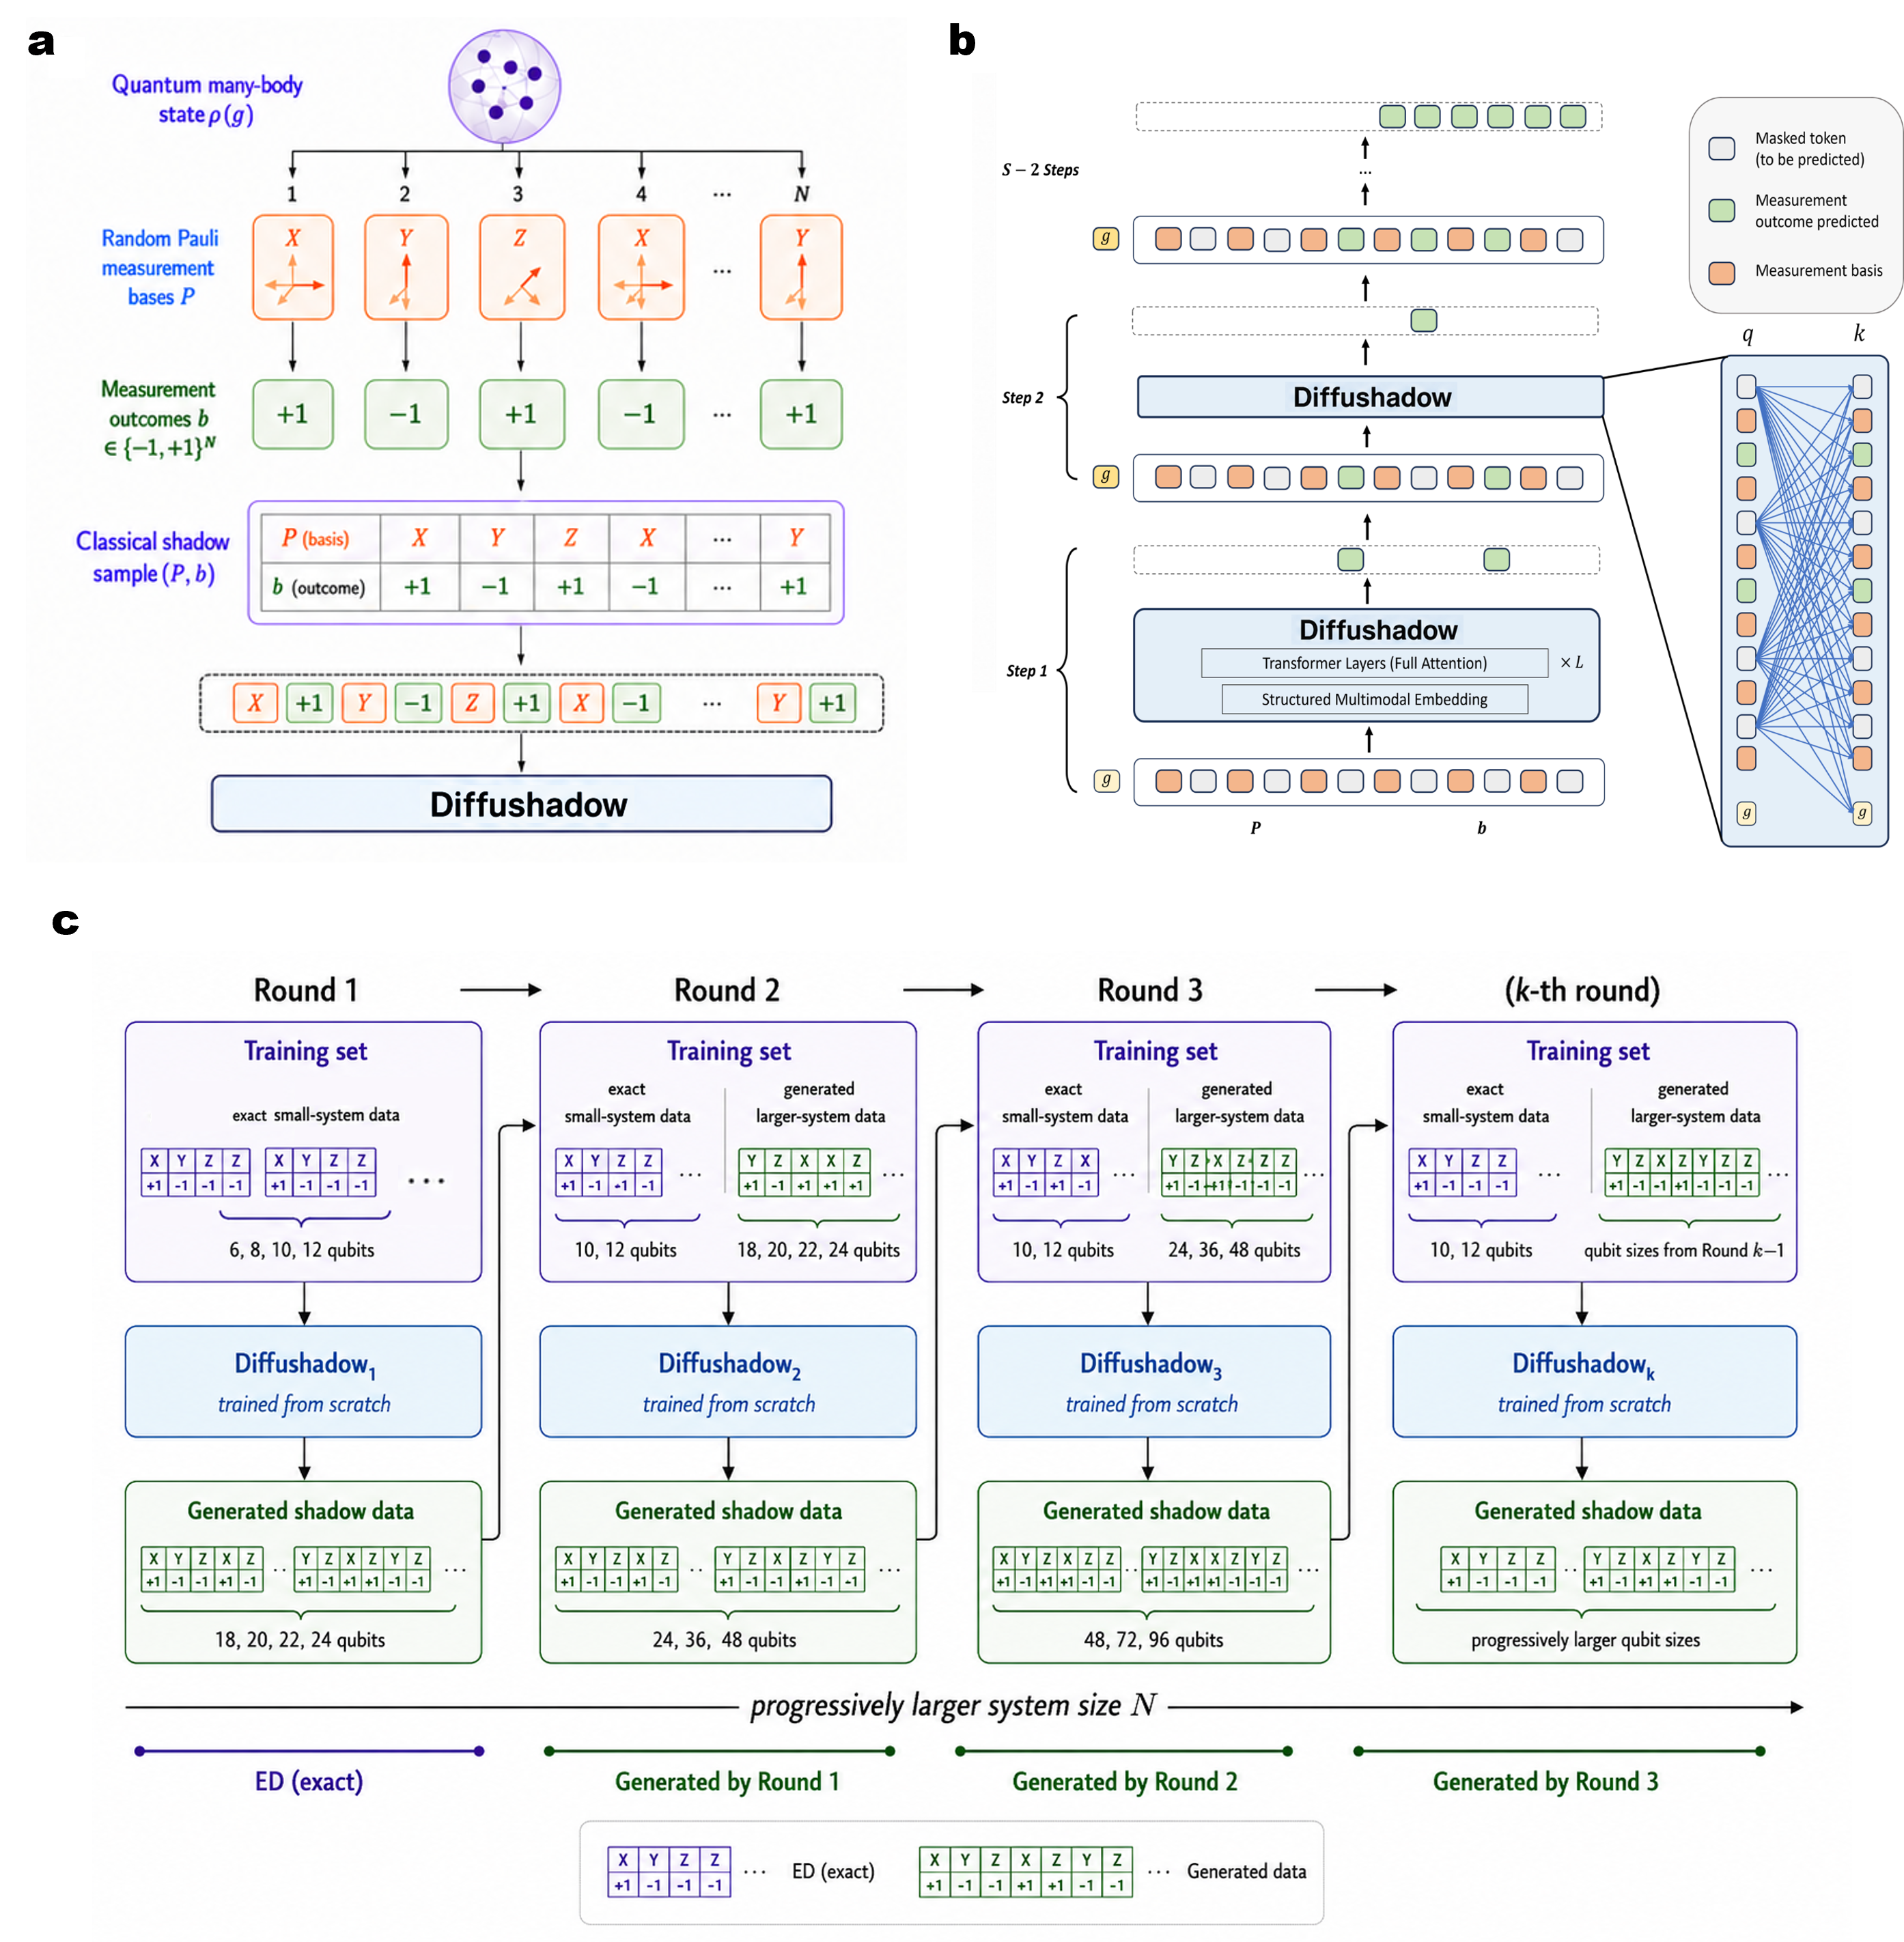
\includegraphics[width=0.98\textwidth]{fig/Figure1_all5.0.png}
\caption{Overview of the Diffushadow framework for scalable quantum measurement generation.
(a) Classical-shadow representation of a quantum many-body state. Each qubit is measured under a randomly selected Pauli basis, and the corresponding measurement outcomes are recorded. The basis sequence $P$ and outcome sequence $b$ together form a classical-shadow snapshot, which is represented as a discrete token sequence for Diffushadow.
(b) Diffusion-based generation of quantum measurement snapshots. Starting from a partially masked measurement sequence, Diffushadow iteratively denoises the configuration and predicts masked measurement outcomes. Full attention allows the model to aggregate information from both measurement-basis and measurement-outcome tokens across the entire sequence, enabling collective refinement without imposing an autoregressive ordering.
(c) Recursive scale extrapolation. Diffushadow is first trained on exact small-system classical-shadow data obtained from exact diagonalization, and is then used to generate shadow data for larger systems beyond the original training sizes. The generated data are incorporated into subsequent training rounds together with the retained exact small-system data, progressively expanding the accessible system size. Purple shadow snapshots denote exact ED data, green shadow snapshots denote generated data, and braces indicate the corresponding qubit numbers.
}\label{fig1}
\end{figure}


\subsubsection{Classical shadow representation}
To efficiently represent quantum many-body systems, we adopt classical shadow tomography \cite{huang2020predicting, aaronson2018shadow} as the measurement representation of Diffushadow. Classical shadows provide a compact and experimentally accessible representation of quantum states by storing randomized measurement outcomes instead of the exponentially large density matrix. As illustrated in Figure \ref{fig1}a, in this framework, each qubit is measured under randomly selected Pauli bases, and the corresponding measurement outcomes collectively form a classical shadow snapshot of the underlying quantum state. By repeatedly performing randomized measurements, classical shadows enable efficient estimation of a wide range of physical observables \cite{huang2021efficient}, including local correlations and many-body properties, from a limited number of measurements. Importantly, classical shadows naturally preserve physically relevant correlation structures while avoiding the exponential complexity associated with wavefunction-based representations. These properties make classical shadows particularly suitable for scalable generative modeling and finite-size scaling analysis toward the thermodynamic limit. 
For Diffushadow, each measurement basis and measurement outcome in a single measurement snapshot is modeled as a token, so a single measurement snapshot constitutes a token sequence. This formulation transforms quantum measurement modeling into a discrete generative learning problem, enabling the diffusion model to directly learn the underlying distribution of quantum measurements from experimentally accessible data. 





\subsubsection{Diffusion generative modeling}

Diffushadow models scalable quantum measurement distributions through a diffusion-based generative paradigm designed to capture global and non-local quantum correlations. To model quantum measurement distributions, Diffushadow employs a full-attention mechanism rather than the causal attention commonly used in autoregressive architectures like GPT. Unlike causal attention, which restricts each prediction to depend only on preceding positions in the sequence, full attention enables bidirectional interactions across the entire quantum measurement configuration as schematically illustrated in the right panel of Figure \ref{fig1}b. The choice of full attention over causal attention is not merely an architectural preference but an alignment with the physical principles governing quantum many-body systems. Quantum systems can exhibit non-local correlations arising from entanglement, and measurement outcomes are not naturally organized as a one-directional causal sequence. 
% Causal attention, with its unidirectional mask, fails to capture correlations with subsequent qubits, artificially breaking the inherent symmetry of quantum entanglement. 
Full attention enables bidirectional information flow, allowing it to model the global, non-local correlations present in quantum many-body systems. 
To further examine the effect of this architectural choice, we performed a causal-mask control experiment. We fixed the measurement outcome of one selected qubit and measured the KL divergence between the predicted distributions of the remaining qubits before and after fixation. As shown in Extended Data Fig.~\ref{fig:kl_divergence_attention}, the causal-attention variant mainly propagates this perturbation to later sequence positions, whereas full-attention Diffushadow allows the perturbation to influence qubits on both sides, consistent with bidirectional information flow.


While full attention provides a mechanism for capturing global correlations within a quantum measurement configuration, Diffushadow further leverages this capability through an iterative denoising process, as illustrated in the left panel of Figure \ref{fig1}b. Unlike autoregressive architectures that generate measurement outcomes sequentially through causal attention, Diffushadow refines all qubits collectively and generates measurement outcomes in no predetermined order during the denoising process. 
% This generative paradigm of Diffushadow enables bidirectional interactions across the entire measurement configuration and allows the model to capture global correlations without imposing an artificial sequential dependency on the generated measurements. 
This design is better aligned with the nature of quantum many-body systems, where measurement outcomes collectively reflect the same underlying quantum state rather than being generated through an intrinsic causal chain. Extended Data Table \ref{tab:mse_table} reports numerical experiments comparing iterative-generation Diffushadow with one-shot generation of all measurement outcomes. The results confirm that iterative generation achieves superior accuracy.
With full attention and iterative denoising, Diffushadow provides an inductive bias for modeling global dependencies in quantum measurement configurations, demonstrating strong potential for effective modeling. Extended Data Table~\ref{tab:mse_table} further compares Diffushadow with the autoregressive ShadowGPT baseline \cite{yao2024shadowgpt}, supporting the effectiveness of full-attention iterative denoising for modeling globally correlated quantum measurement configurations.

% In addition to full attention, Diffushadow generates quantum measurements through iterative denoising. Unlike autoregressive architectures that generate measurement outcomes sequentially in a predetermined order, Diffushadow collectively refines all qubits during the denoising process. This generative paradigm allows all measurement outcomes to emerge simultaneously from the same underlying quantum state rather than through an artificial sequential dependency. By enabling collective refinement across the entire system, Diffushadow more effectively captures global and long-range quantum correlations in scalable quantum many-body systems.



\begin{figure}[ht]
\centering
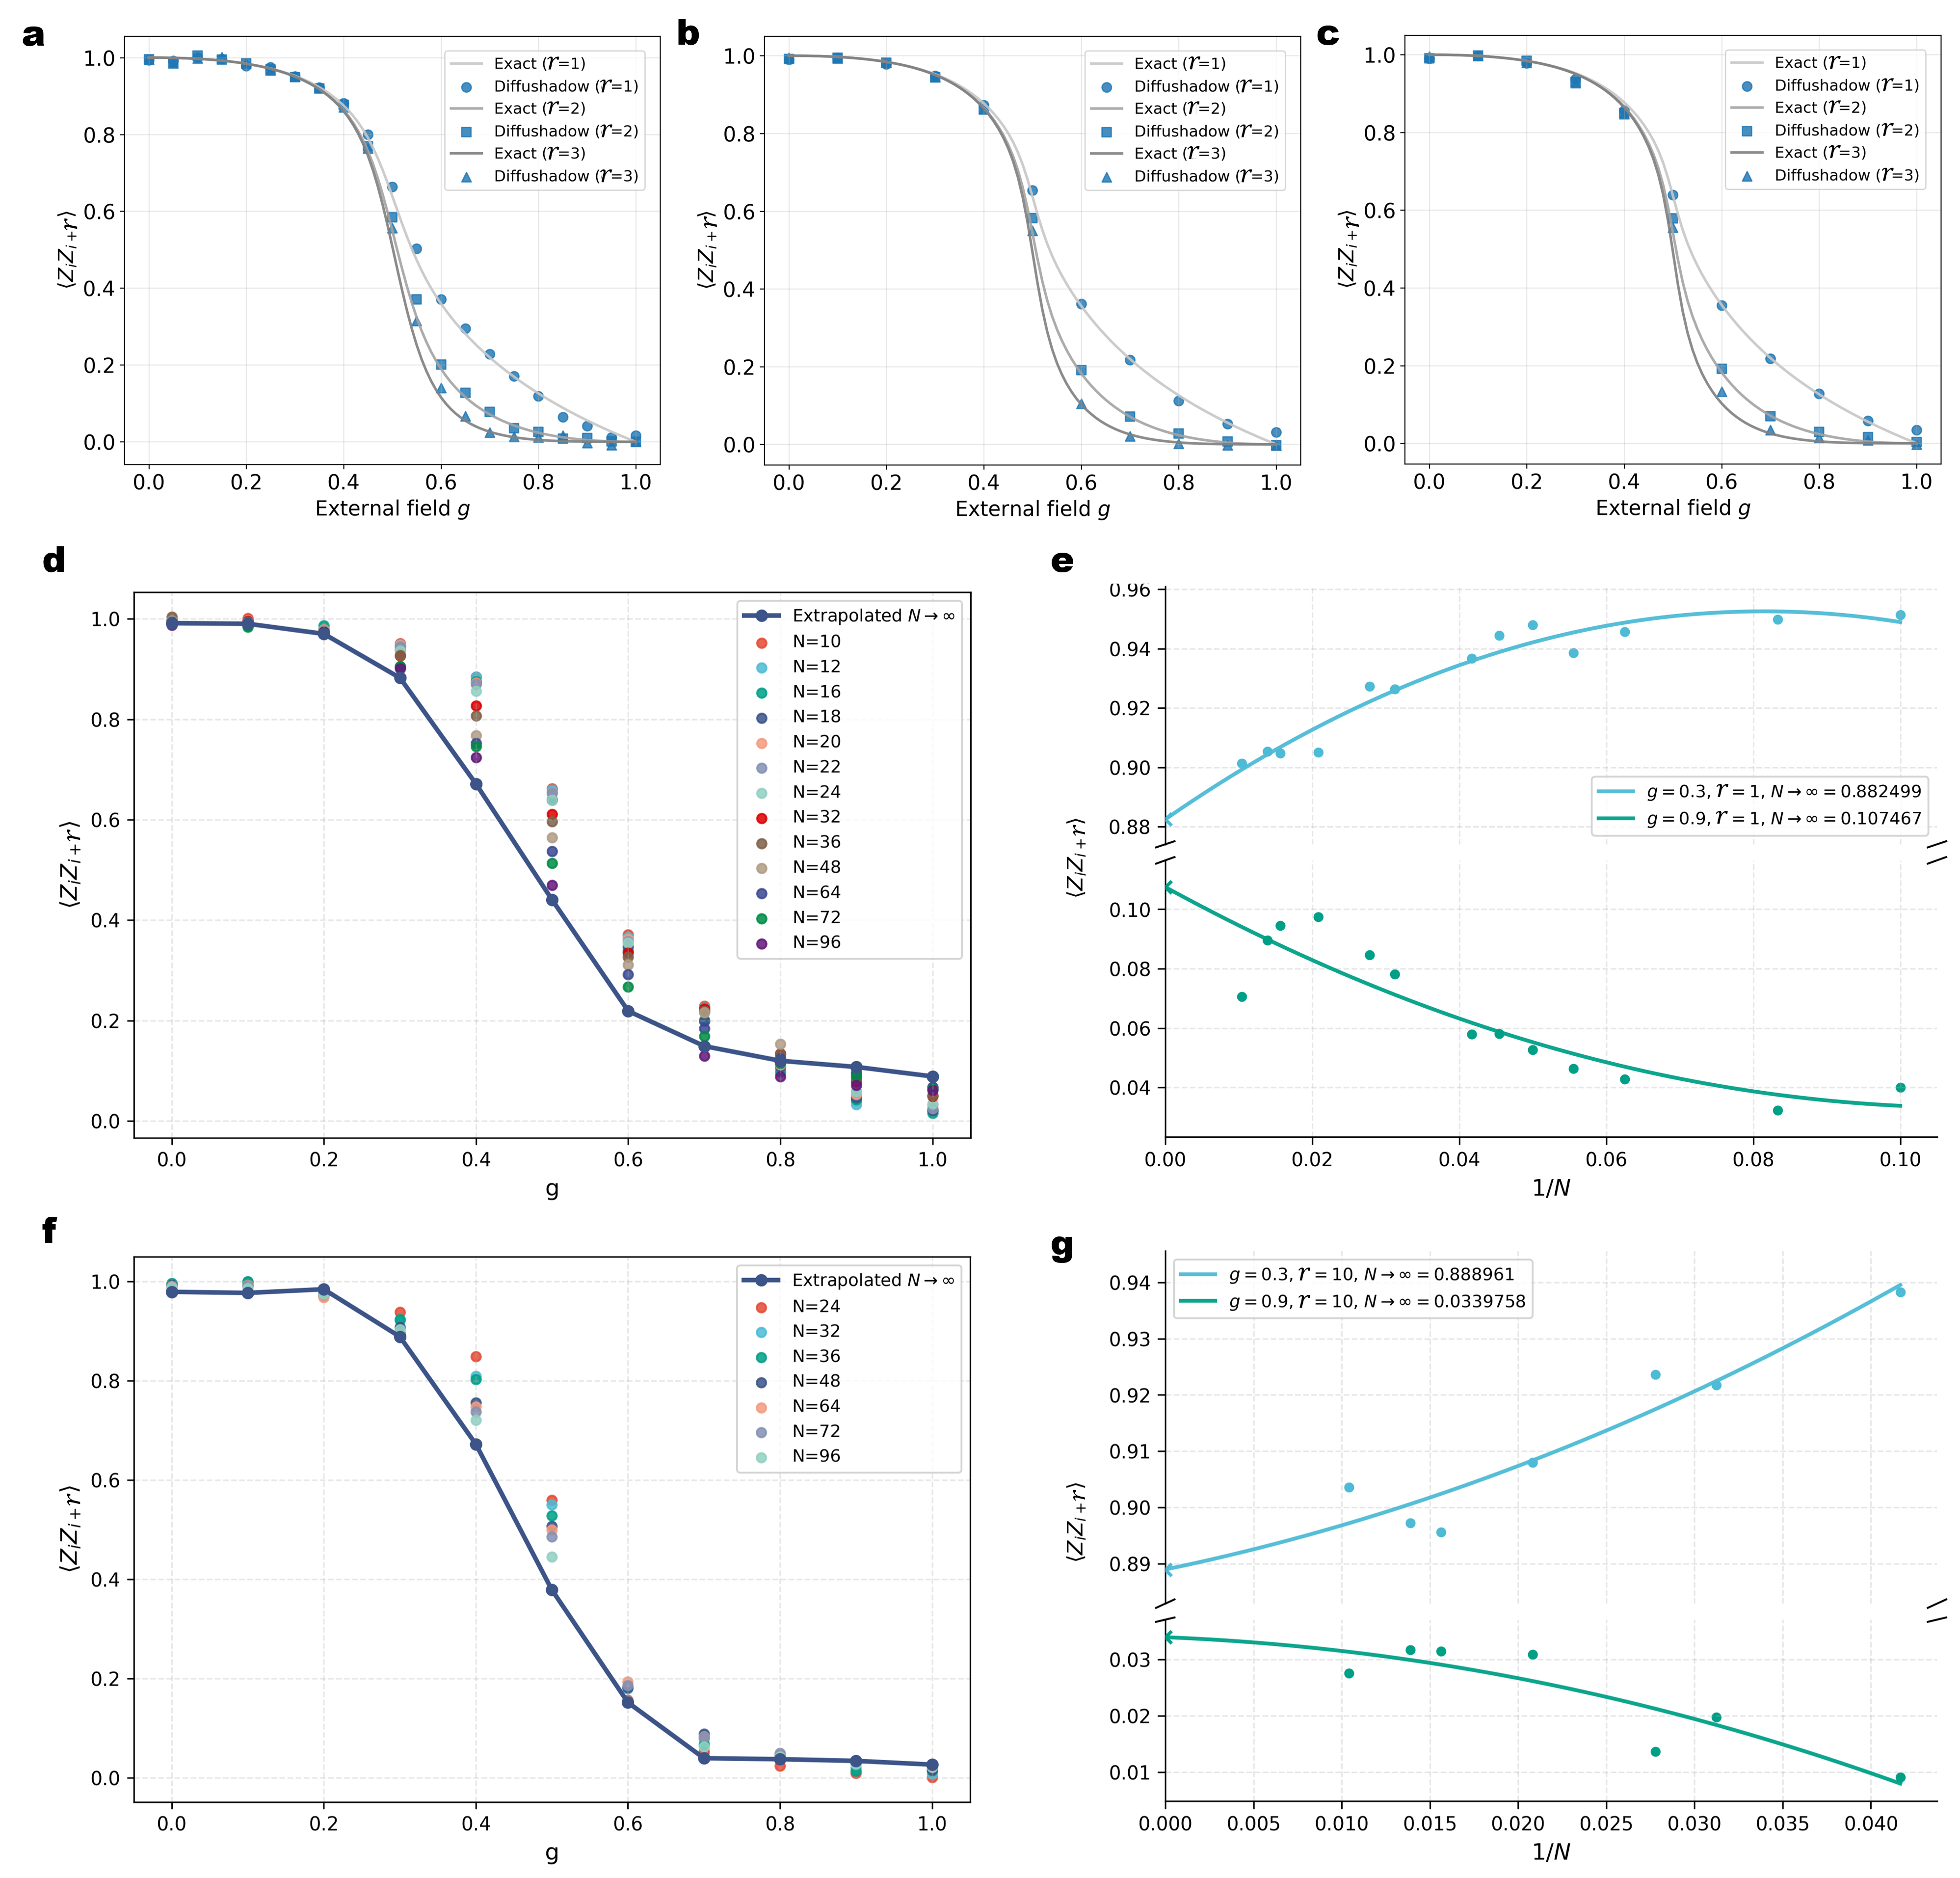
\includegraphics[width=0.98\textwidth]{fig/Figure_TFI_all1.2.png}
\caption{Diffushadow enables cross-scale measurement generation and thermodynamic-limit inference in the transverse-field Ising model. 
(a) Same-size generation results for the 10-qubit transverse-field Ising model. 
(b,c) Cross-scale generation results for 20- and 24-qubit systems generated by Diffushadow models trained only on smaller systems. 
In (a--c), exact diagonalization results are shown as solid lines, while blue markers denote physical observables estimated from Diffushadow-generated classical-shadow measurements. Results are shown for spin-spin correlations $\langle Z_i Z_{i+r} \rangle$ with $r=1,2,3$. 
(d,f) Thermodynamic-limit correlation profiles for $r=1$ and $r=10$ obtained by extrapolating finite-size estimates to $N\to\infty$. 
(e,g) Representative finite-size scaling curves for $r=1$ and $r=10$ at $g=0.3$ and $g=0.9$. The observables are fitted as functions of $1/N$ and extrapolated to $1/N=0$, yielding estimates in the thermodynamic limit.}\label{fig2}
\end{figure}


% \subsubsection{Validation across representative spin-chain Hamiltonians}

% We conducted experiments on Diffushadow to verify whether it can effectively model the measurement data of quantum many-body systems. We begin by validating Diffushadow on finite-size instances of representative one-dimensional quantum spin-chain Hamiltonians, ranging from the transverse-field Ising model \cite{pfeuty1970one} to frustrated and competing-interaction models such as the $J_1$-$J_2$ chain \cite{majumdar1969next, majumdar1969next2} and the axial next-nearest-neighbor Ising (ANNNI) model \cite{selke1988annni}. These models cover both a canonical quantum phase-transition benchmark and spin-chain systems with competing interactions, providing a testbed for assessing whether Diffushadow can model quantum measurement distributions beyond a single Hamiltonian. For each Hamiltonian, Diffushadow is trained on small-system classical-shadow measurements and used to generate measurement snapshots of the same size. Physical observables estimated from the generated measurements are then compared with exact results. Figure \ref{fig2} a-c present the ground state property estimated by the data generated by Diffushadow for the transverse-field Ising model, the $J_1$-$J_2$ model, and the ANNNI model, respectively. We focus on the correlation function $<Z_iZ_{i+r}>, r=1,...,5$ of order parameters. In the figure, solid lines correspond to exact diagonalization results, and blue scattered points indicate predictions made by Diffushadow. It is evident that Diffushadow's estimates closely align with the exact solutions across the parameter $g$. This suggests that our model attains a high degree of predictive accuracy. On the other hand, considering our model is trained on a few different sparse values of $g$, the results show that our model exhibits promising generalization capabilities. This is significant for the efficient generation of a large amount of shadow data with diverse $g$ values. 
% These results demonstrate that Diffushadow generates measurements that reproduce key ground-state observables at trained system sizes, providing a foundation for accurate physical-property estimation.




% We next examine whether the learned measurement structures can transfer to larger systems not observed during training. For this purpose, Diffushadow is trained on mixed-size measurement data from smaller systems and then used to generate measurements for larger target systems. Figures~\ref{fig2}d--f and \ref{fig2}g--i present cross-size generation results for 20- and 24-qubit systems, respectively. Within each row, the three panels correspond to the transverse-field Ising model, the \(J_1\)-\(J_2\) model, and the ANNNI model. The generated-measurement estimates remain close to the exact results across these larger system sizes, indicating that Diffushadow can generalize beyond the system sizes used during training in these spin-chain settings. This behavior is consistent with the model learning measurement structures that are transferable across finite-size instances, rather than relying solely on size-specific training patterns.



\subsection{Cross-scale generation and thermodynamic-limit inference in the TFI model}

% We have demonstrated that Diffushadow is capable of learning transferable quantum structures and generalizing to larger quantum many-body systems. However, direct zero-shot extrapolation alone remains insufficient for approaching the thermodynamic limit. To further extend the accessible system size of Diffushadow, we introduce a recursive scale extrapolation procedure, which is a progressive scale-expansion framework for quantum measurement generation. This process begins with Diffushadow being trained on a mixed dataset of accurately generated measurement data from several small-scale quantum many-body systems. Then, we employ the trained Diffushadow to produce measurement data for larger-scale quantum many-body systems, thereby completing the first round of iteration. In the second round of training, Diffushadow is trained from scratch using the data generated in the first round along with a portion of the accurate data used in the first round. Similar to the first round, in the second round Diffushadow again generates quantum many-body data of a larger scale than the data it was trained on. All subsequent rounds proceed in the same manner. It is worth noting that the only exact data used throughout the entire process are the small-scale quantum many-body data employed in the first round of training. This is largely due to the fact that data from smaller quantum systems are both easily accessible and highly accurate.

Having introduced the iterative denoising framework of Diffushadow, we next evaluate whether this generative model can support scalable quantum measurement inference beyond the system sizes used for training. We first focus on the transverse-field Ising model as a controlled benchmark, because it provides a simple but physically nontrivial setting with a well-characterized transition between ferromagnetic and paramagnetic regimes. This allows us to assess not only whether Diffushadow can reproduce finite-size measurement statistics, but also whether the generated measurements can be used for cross-scale extrapolation and thermodynamic-limit inference. In this section, we use longitudinal spin correlations \(\langle Z_i Z_{i+r}\rangle\) as representative physical observables and present the full inference pipeline in Fig.~\ref{fig2}, including same-size measurement generation, cross-scale generation to larger unseen systems, recursive scale extrapolation, and finite-size scaling toward the thermodynamic limit.



\subsubsection{Cross-scale measurement generation in the TFI model}

Before using generated measurements for thermodynamic-limit inference, we first assess whether Diffushadow can reproduce finite-size transverse-field Ising observables both within and beyond the training system sizes.

We begin by examining same-size measurement generation in the transverse-field Ising model, where Diffushadow is trained and evaluated on 10-qubit systems. This setting provides a direct test of whether the learned generative model can reproduce physical observables from classical-shadow measurement samples at system sizes included in training. As shown in Fig.~\ref{fig2}a, spin-spin correlation functions \(\langle Z_i Z_{i+r}\rangle\) estimated from Diffushadow-generated measurements closely follow the exact diagonalization results across the scanned transverse-field parameter \(g\). These results indicate that Diffushadow can generate measurement samples that preserve the longitudinal correlation structure of the transverse-field Ising ground state at training system sizes. The corresponding mean squared errors between Diffushadow estimates and exact results are reported in Extended Data Table~\ref{tab:mse_table}.

Beyond faithfully modeling quantum measurements within the training regime, an important question is whether Diffushadow can generalize the learned quantum measurement structures to larger quantum systems that are inaccessible during training. To investigate this question, Diffushadow is trained on mixed-size measurement data from smaller systems and then used to generate measurements for larger target systems that were never observed during training. 
By exposing the model to measurements from multiple scales during training, Diffushadow is encouraged to learn quantum structures that are shared across system sizes rather than size-specific patterns tied to a particular finite system.
Figures \ref{fig2}b--c present the cross-scale generation results for 20- and 24-qubit systems, respectively, all of which exceed the system sizes used during training. In these figures, the generated-measurement estimates remain close to the exact results, indicating that Diffushadow can generalize to larger unseen system sizes in these spin-chain settings. This suggests that Diffushadow does not merely reproduce size-specific training measurement patterns, but instead learns transferable quantum structures that persist across system scales. These learned structures enable the model to extrapolate beyond the original training regime and generate physically meaningful quantum measurements for larger many-body systems.


\subsubsection{Thermodynamic-limit inference from recursively generated measurements}


We have demonstrated that Diffushadow is capable of learning transferable quantum structures and generalizing to larger quantum many-body systems. However, direct zero-shot extrapolation alone remains insufficient for approaching the thermodynamic limit. To further extend the accessible system size of Diffushadow, we introduce a recursive scale extrapolation procedure, which is a progressive scale-expansion framework for quantum measurement generation, as shown in Figure \ref{fig1}c.
The procedure begins with Diffushadow being trained on a mixed dataset consisting of accurate measurement data from several small-scale quantum many-body systems. The trained model is then used to generate measurement data for larger systems beyond the original training regime. These generated measurements are subsequently incorporated into the training data for the next round, enabling the model to progressively expand its accessible system size. By iteratively repeating this process, Diffushadow progressively transfers the learned quantum measurement structures to increasingly larger quantum many-body systems. The stability of this recursive procedure is further examined in Supplementary Fig.4, where 24-qubit observables generated by Diffushadow models from different recursive rounds remain largely consistent, suggesting that the recursive training process does not introduce substantial drift at the tested scale.
% To assess the stability of recursive scale extrapolation, we further compare 24-qubit predictions from Diffushadow models trained in different recursive rounds in the Supplementary Information. The predictions remain largely consistent across rounds, suggesting that incorporating generated measurements into subsequent training stages does not introduce substantial drift or error accumulation in this setting.
% Instead, the learned quantum structures remain remarkably stable throughout the recursive expansion process, allowing Diffushadow to consistently reproduce physically meaningful quantum measurements at scales beyond the original training regime.
Importantly, the only exact data required throughout the entire recursive extrapolation process are the small-scale quantum measurements used during the initial training stage. All subsequent generations are derived from the recursively expanded models, allowing the accessible system size to grow far beyond that of the original training data. This reduces the dependence on large-scale exact measurements, which are often prohibitively expensive to obtain from either numerical simulations or quantum experiments.

As a result, recursive scale extrapolation provides a practical pathway for extending quantum measurement modeling toward system sizes that would otherwise remain inaccessible, thereby enabling thermodynamic-limit inference from a small set of exact measurements together with recursively generated large-scale quantum data.


\begin{figure}[ht]
\centering
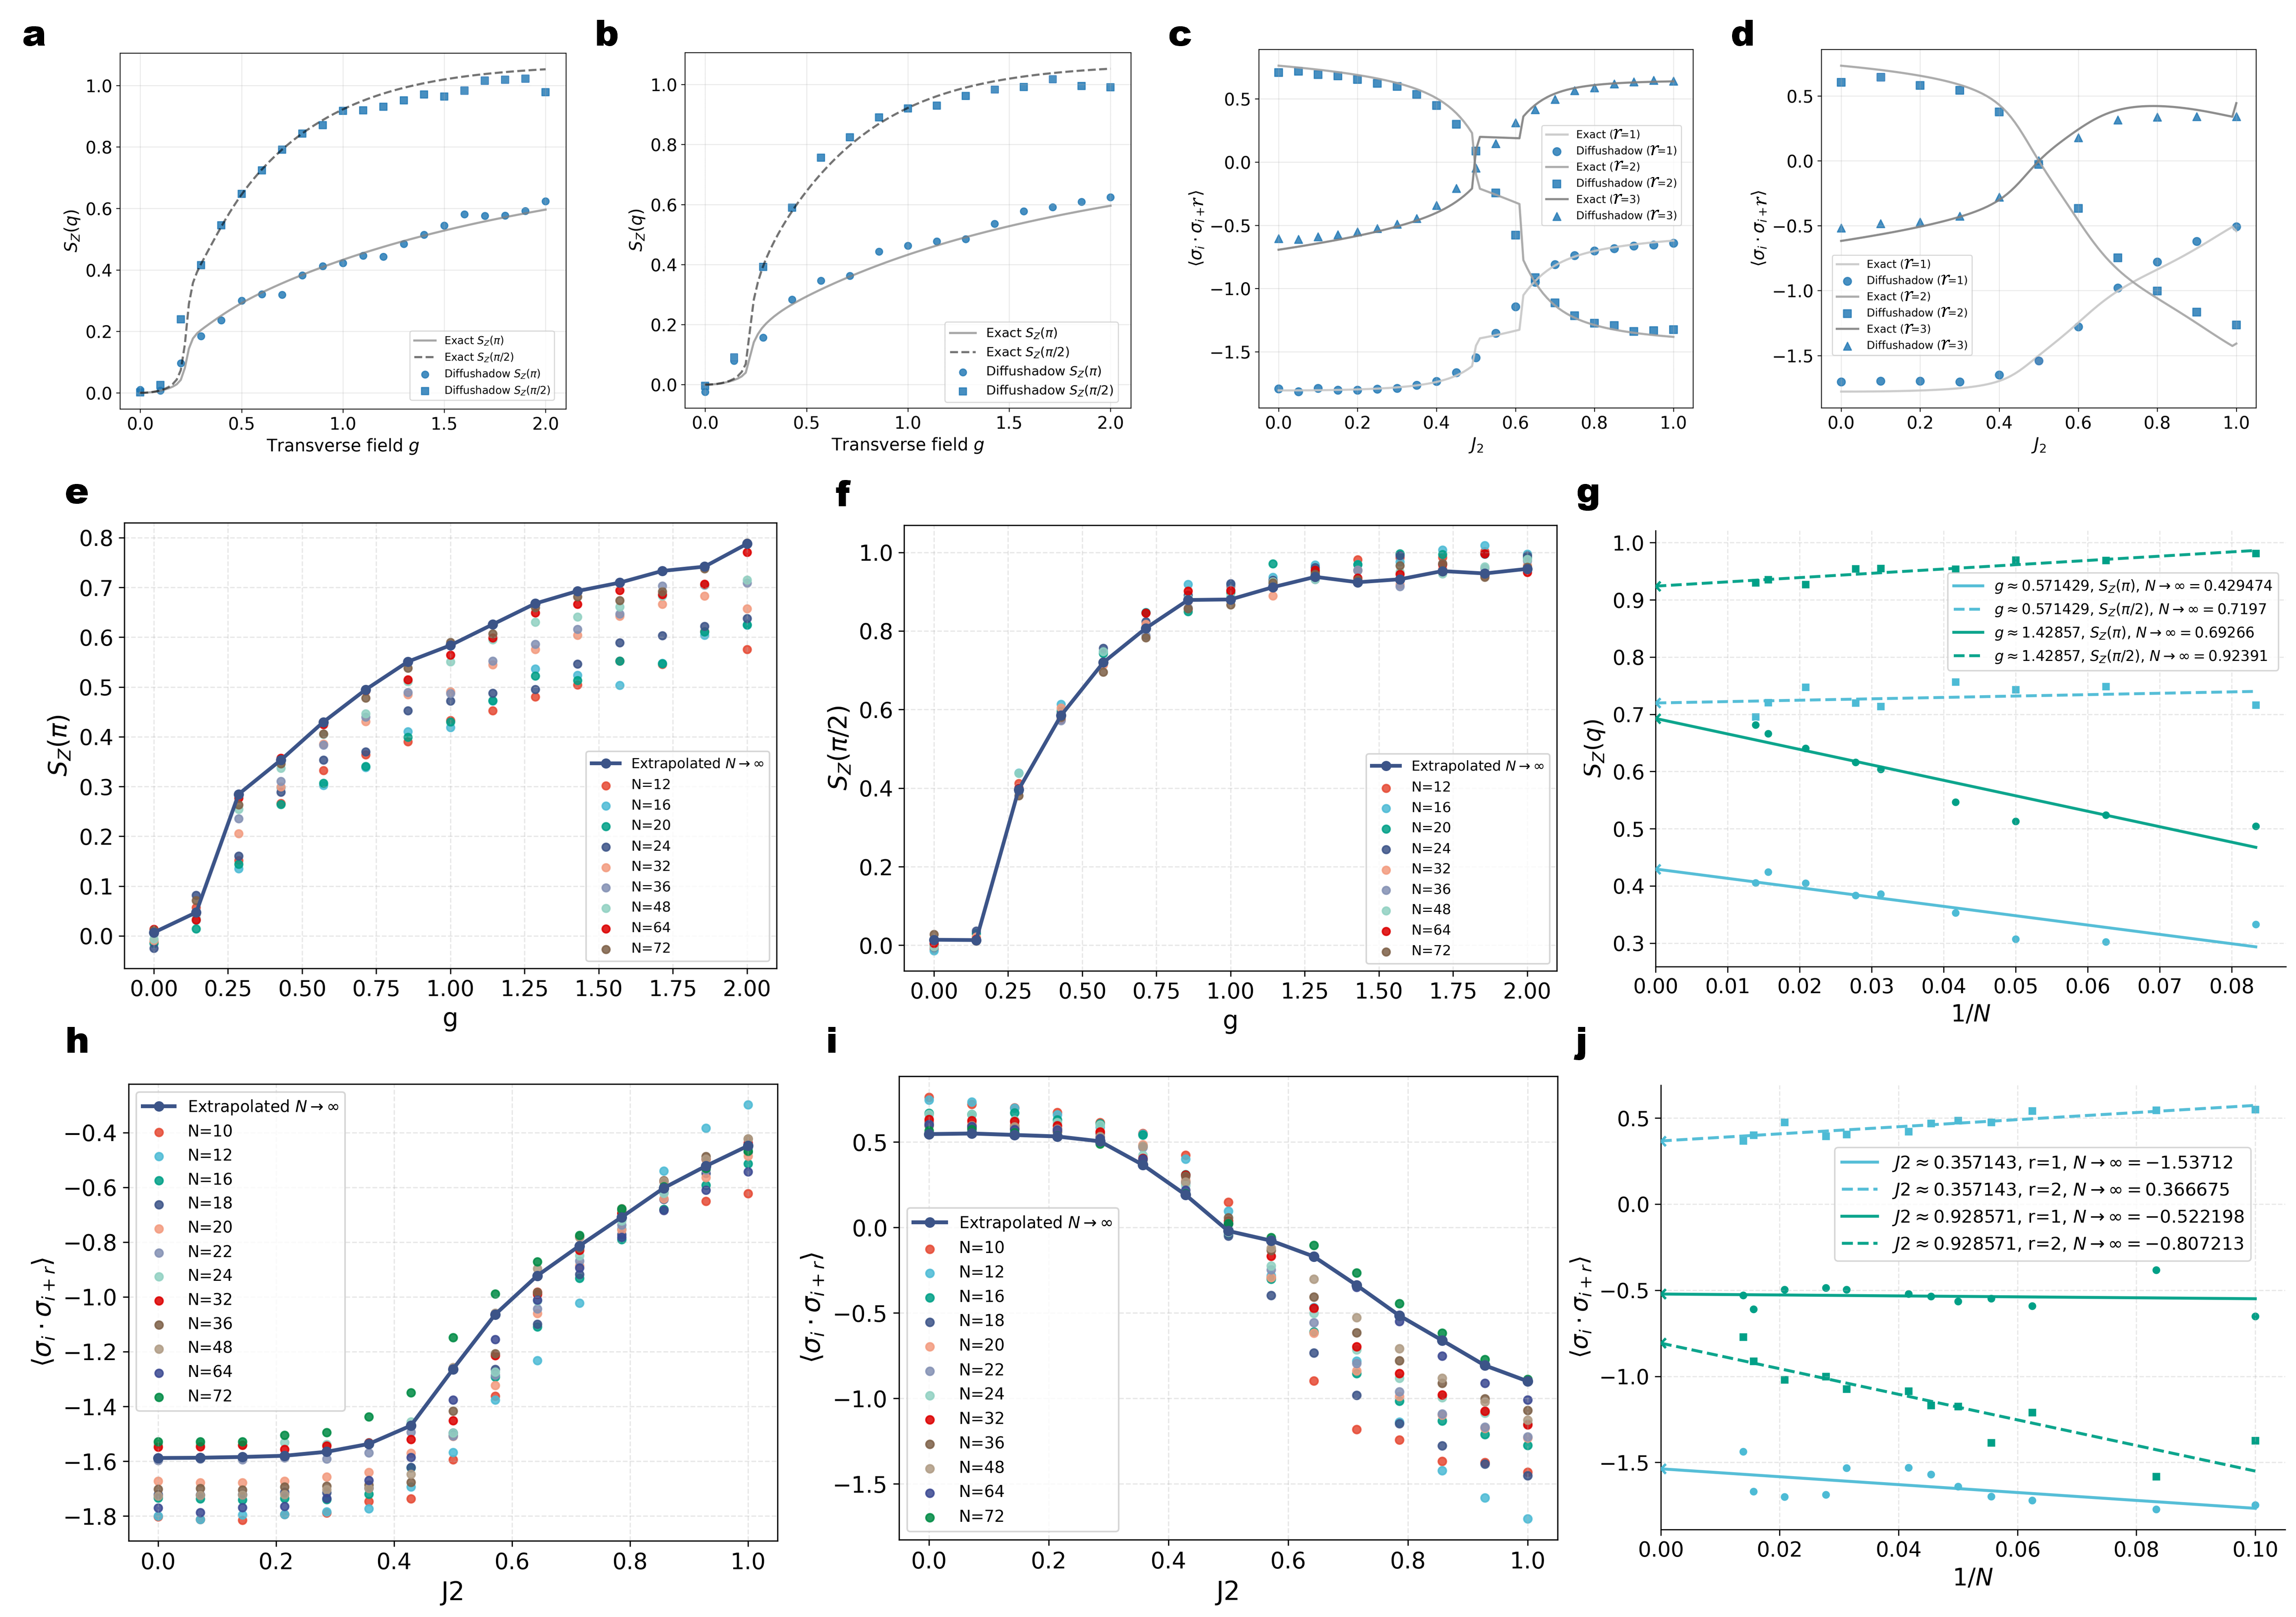
\includegraphics[width=\textwidth]{fig/Figure_ANNNI_J1J2_all3.0.png}
\caption{Cross-scale generation and thermodynamic-limit inference in frustrated and competing-interaction spin chains.
(a,b) Measurement-generation results for the ANNNI model at 12 and 24 qubits, respectively. The structure factors \(S_Z(\pi)\) and \(S_Z(\pi/2)\) estimated from Diffushadow-generated classical-shadow measurements are compared with exact diagonalization results as functions of the transverse-field parameter \(g\). 
(c,d) Measurement-generation results for the $J_1$-$J_2$ model at 10 and 24 qubits, respectively. Spin-dot correlations \(\langle \boldsymbol{\sigma}_i\cdot\boldsymbol{\sigma}_{i+r}\rangle\) with \(r=1,2,3\) are shown as functions of the frustration parameter \(J_2\). 
(e,f) Thermodynamic-limit inference of the ANNNI structure factors \(S_Z(\pi)\) and \(S_Z(\pi/2)\), obtained by extrapolating finite-size estimates to \(N\to\infty\). 
(g) Representative finite-size scaling curves for ANNNI observables, where structure factors estimated from finite systems are fitted as functions of \(1/N\) and extrapolated to \(1/N=0\). 
(h,i) Thermodynamic-limit inference of the $J_1$-$J_2$ spin-dot correlations for \(r=1\) and \(r=2\), respectively. 
(j) Representative finite-size scaling curves for $J_1$-$J_2$ spin-dot correlations at selected values of \(J_2\). 
In all panels, solid or dashed curves denote exact results or fitted extrapolation curves, while markers denote observables estimated from Diffushadow-generated classical-shadow measurements. These results show that Diffushadow preserves model-specific ordering and correlation structures beyond the transverse-field Ising model and supports finite-size extrapolation in frustrated and competing-interaction spin chains.}\label{fig3}
\end{figure}



Having established the ability of Diffushadow to generate physically consistent quantum measurements at scales far beyond the original training regime, we next seek to infer physical properties in the thermodynamic limit. We focus on the spin-spin correlation function $\langle Z_i Z_{i+r} \rangle$, a fundamental observable for characterizing quantum phases and correlation structures in the transverse-field Ising model.

The large-scale quantum measurements generated through recursive scale extrapolation provide access to system sizes that would otherwise be inaccessible using the original training data alone. Following the standard finite-size scaling paradigm in many-body physics, observables extracted from the generated measurements are analyzed as functions of the inverse system size $1/N$ \cite{privman1990finite, cardy1996scaling}. The resulting scaling curves are then extrapolated to the limit $1/N \rightarrow 0$, corresponding to the thermodynamic limit $N \rightarrow \infty$. This enables thermodynamic-limit properties to be estimated from a combination of exact and Diffushadow-generated quantum measurements spanning a broad range of system sizes.

Figures~\ref{fig2}e and g show the finite-size scaling of \(\langle Z_i Z_{i+r}\rangle\), estimated from Diffushadow-generated measurements, for different correlation distances \(r\) in the ferromagnetic (\(g=0.3\)) and paramagnetic (\(g=0.9\)) regimes, respectively.
% Figure \ref{fig3} e and g display how $\langle Z_i Z_{i+r}\rangle$ generated by Diffushadow varies with $1/N$ for different correlation distance $r$, in the ferromagnetic $g = 0.3$ and paramagnetic $g = 0.9$ phases, respectively.
For each correlation distance, observables extracted from both exact and Diffushadow-generated measurements exhibit smooth dependence on the inverse system size $1/N$. Finite-size fits in $1/N$ effectively capture the finite-size corrections and provide stable estimates of the corresponding thermodynamic-limit values by extrapolating to $1/N=0$.

Extrapolation across a range of $g$ values yields the thermodynamic-limit correlation profiles for distances $r = 1$ and $10$, presented in Figures~\ref{fig2}d and f. Several notable trends can be observed from the extrapolated thermodynamic-limit correlation profiles. In the ferromagnetic regime ($g<0.5$), the thermodynamic-limit correlations are generally slightly smaller than the corresponding finite-size estimates. This deviation becomes substantially more pronounced near the critical region ($g\approx0.5$), where the extrapolated values lie noticeably below those obtained for the largest accessible finite systems. In contrast, in the paramagnetic regime ($g>0.5$), the extrapolated thermodynamic-limit correlations are typically slightly larger than their finite-size counterparts.




\subsection{Generalization to frustrated and competing-interaction spin chains}


% Through recursive scale extrapolation, the Diffushadow models trained across different rounds produce quantum many-body data at progressively larger system sizes. These data then enable the estimation of physical properties for quantum systems in the thermodynamic limit. Following the standard finite-size scaling paradigm in many-body physics, observables extracted from the generated measurements are analyzed as functions of the inverse system size $1/N$. Extrapolating the resulting scaling curves to $1/N=0$ provides estimates of their thermodynamic-limit values, allowing physical properties beyond the accessible finite-size regime to be inferred directly from Diffushadow-generated data.



% As shown in Fig. XX, the availability of large-scale quantum measurements generated through recursive scale extrapolation enables the construction of finite-size scaling curves over a substantially broader range of system sizes than would be accessible from exact data alone. For each correlation distance ($r$), spin-spin correlations $(\langle Z_i Z_{i+r}\rangle)$ estimated from both exact and generated measurements exhibit smooth and systematic dependence on the inverse system size ($1/N$). To capture the finite-size corrections and infer the corresponding thermodynamic-limit values, we fit the scaling curves using quadratic functions of ($1/N$) and extrapolate them to ($1/N=0$).

After establishing the full cross-scale generation and thermodynamic-limit inference pipeline in the transverse-field Ising model, we next examine whether Diffushadow can be extended beyond this canonical benchmark. To this end, we consider two representative one-dimensional spin-chain Hamiltonians with more complex interaction structures: the frustrated \(J_1\)-\(J_2\) model and the axial next-nearest-neighbor Ising (ANNNI) model. The \(J_1\)-\(J_2\) model introduces competing nearest- and next-nearest-neighbor exchange interactions and exhibits frustration-induced dimerization physics, while the ANNNI model contains competing Ising interactions that give rise to modulated ordering tendencies. These models therefore provide a broader testbed for assessing whether Diffushadow can generate physically meaningful quantum measurement samples and support finite-size extrapolation beyond the transverse-field Ising setting.


Because the characteristic physics of these Hamiltonians is different from that of the transverse-field Ising model, we evaluate model-specific observables that directly reflect their dominant interactions and ordering tendencies. For the \(J_1\)-\(J_2\) model, we focus on the spin-dot correlations
\(\langle \boldsymbol{\sigma}_i \cdot \boldsymbol{\sigma}_{i+r} \rangle\). In the finite-size generation tests, we use \(r=1,2,3\) to assess whether Diffushadow captures the nearest-neighbor, next-nearest-neighbor, and longer-distance correlation structures. For thermodynamic-limit inference, we focus on \(r=1\) and \(r=2\), which directly correspond to the two exchange terms in the \(J_1\)-\(J_2\) Hamiltonian. For the ANNNI model, we evaluate the structure factors \(S_Z(\pi)\) and \(S_Z(\pi/2)\), which probe distinct ordering tendencies associated with competing Ising interactions. In particular, \(S_Z(\pi/2)\) is sensitive to modulated ordering with period-four character, while \(S_Z(\pi)\) captures staggered ordering components. These observables therefore provide compact but physically meaningful tests of whether Diffushadow-generated measurements preserve the relevant correlation and ordering structures beyond the transverse-field Ising model.

We first evaluate finite-size measurement generation for these two Hamiltonians. Figures~\ref{fig3}a,b show the ANNNI results at 12 and 24 qubits, corresponding to same-size and cross-scale generation, respectively. The structure factors \(S_Z(\pi)\) and \(S_Z(\pi/2)\) estimated from Diffushadow-generated measurements are in good agreement with the exact results across the transverse-field parameter \(g\). For both system sizes, the generated measurements reproduce the distinct evolution of the two ordering components, including the rapid growth of \(S_Z(\pi/2)\) and the more gradual variation of \(S_Z(\pi)\). Figures~\ref{fig3}c,d show the corresponding results for the \(J_1\)-\(J_2\) model at 10 and 24 qubits, representing same-size and cross-scale generation, respectively. Diffushadow captures the main evolution of the spin-dot correlations at \(r=1,2,3\) as the frustration parameter \(J_2\) is varied, including the contrasting trends of correlations at different distances. These results show that Diffushadow can generate measurement samples that preserve model-specific correlation and ordering structures not only at training system sizes, but also during cross-scale generation to larger spin chains.


We next examine whether the generated measurements for these more complex spin chains can also support finite-size extrapolation. Following the recursive scale-extrapolation strategy used for the transverse-field Ising model, we generate classical-shadow measurements for a sequence of larger system sizes and estimate the corresponding model-specific observables. These finite-size estimates are then analyzed as functions of \(1/N\) and extrapolated to \(1/N=0\), yielding thermodynamic-limit estimates for the selected observables.

For the ANNNI model, Figures~\ref{fig3}e and \ref{fig3}f show the extrapolated thermodynamic-limit profiles of the structure factors \(S_Z(\pi)\) and \(S_Z(\pi/2)\), respectively. The finite-size estimates obtained from Diffushadow-generated measurements exhibit systematic size dependence, while the extrapolated curves remain physically smooth across the transverse-field parameter \(g\). The resulting thermodynamic-limit estimates preserve the distinct behavior of the two ordering components: \(S_Z(\pi/2)\) displays a rapid growth and approaches a large value over a broad large-\(g\) region, whereas \(S_Z(\pi)\) varies more gradually with \(g\). Representative finite-size scaling curves are shown in Fig.~\ref{fig3}g, where the observables estimated from different system sizes follow smooth trends as functions of \(1/N\) and can be extrapolated to the thermodynamic limit.

For the $J_1$-$J_2$ model, Figures~\ref{fig3}h and \ref{fig3}i present the corresponding thermodynamic-limit estimates of the spin-dot correlations \(\langle \boldsymbol{\sigma}_i\cdot\boldsymbol{\sigma}_{i+r}\rangle\) for \(r=1\) and \(r=2\). These two distances directly probe the nearest-neighbor and next-nearest-neighbor exchange terms in the Hamiltonian. The extrapolated \(r=1\) correlation increases from a strongly negative value as \(J_2\) grows, while the \(r=2\) correlation shows a contrasting evolution and changes sign as the frustration parameter is varied. These trends are consistent with the competition between nearest- and next-nearest-neighbor interactions in the $J_1$-$J_2$ chain. Representative scaling curves in Fig.~\ref{fig3}j further show that the generated-measurement estimates at different system sizes can be organized by finite-size scaling in \(1/N\), enabling extrapolation of the spin-dot correlations toward \(N\to\infty\).

Together, these results extend the thermodynamic-limit inference pipeline beyond the transverse-field Ising benchmark. Although the frustrated $J_1$-$J_2$ and ANNNI models exhibit more complex finite-size behavior, Diffushadow-generated measurements still preserve the relevant model-specific correlation and ordering structures across system sizes. This supports the use of Diffushadow as a flexible measurement-generation framework for finite-size extrapolation in one-dimensional spin-chain systems with competing interactions.


% Figures~\ref{fig3}c,d show the corresponding results for the \(J_1\)-\(J_2\) model at 10 and 24 qubits, representing same-size and cross-scale generation, respectively. We evaluate the spin-dot correlations \(\langle \boldsymbol{\sigma}_i\cdot\boldsymbol{\sigma}_{i+r}\rangle\) at distances \(r=1,2,3\). As the frustration parameter \(J_2\) increases, the nearest-neighbor correlation becomes less negative, while the next-nearest-neighbor correlation decreases and changes sign. The third-neighbor correlation exhibits an opposite trend, increasing from negative to positive values. Diffushadow-generated measurements reproduce these distance-dependent trends in both the trained-size and cross-scale settings, indicating that the model can capture the redistribution of spin correlations induced by competing exchange interactions.



\subsection{Learning physically aligned quantum structures}

% Although Diffushadow exhibits promising performance in generalizing towards large-scale quantum systems, a crucial question remains: Does Diffushadow genuinely comprehend the physical implications of the many-body system and learn transferable quantum structures?

Although Diffushadow exhibits strong performance in modeling and generalizing quantum measurement distributions across system sizes, it remains important to ask whether its cross-scale behavior is supported by physically meaningful internal structures rather than by memorization of finite-size statistical patterns. We investigate this question in the transverse-field Ising model, which provides a controlled setting with well-characterized phases and exact spin-spin correlation profiles. Through attention analysis, we investigate the internal structures learned by the model \cite{clark2019does}, thereby providing a mechanistic perspective on Diffushadow's scale generalization. 



We first quantify the spatial range of attention by measuring the attention-weighted site distance from masked measurement queries to site-indexed tokens. Specifically, we compute the average distance between a masked measurement token and the sites it attends to, weighted by attention scores and averaged over all masked queries, heads and layers. Here, site-indexed tokens include both measurement-basis tokens $P_i$ and measurement-outcome tokens $b_i$. Intuitively, this quantity measures the effective spatial receptive field of the model. Higher values indicate that information is aggregated from more distant sites, whereas lower values imply a stronger reliance on local neighborhoods. As shown in Figure \ref{fig4}a, the normalized mean site distance varies systematically with the coupling parameter, indicating that the model adapts its spatial receptive field across physical regimes. Moreover, it remains consistently larger in the ordered regime ($g<0.5$) than in the paramagnetic regime ($g>0.5$) across all system sizes. This trend is consistent with the physical characteristics of the one-dimensional transverse-field Ising model, where the ferromagnetic phase is associated with stronger and more extended spatial correlations, while correlations become increasingly short-ranged in the paramagnetic phase. Notably, the overall shape of the curves remains highly consistent across different system sizes, suggesting that the model captures scale-invariant features of the underlying quantum system rather than memorizing size-specific patterns. 


\begin{figure}[ht!]
\centering
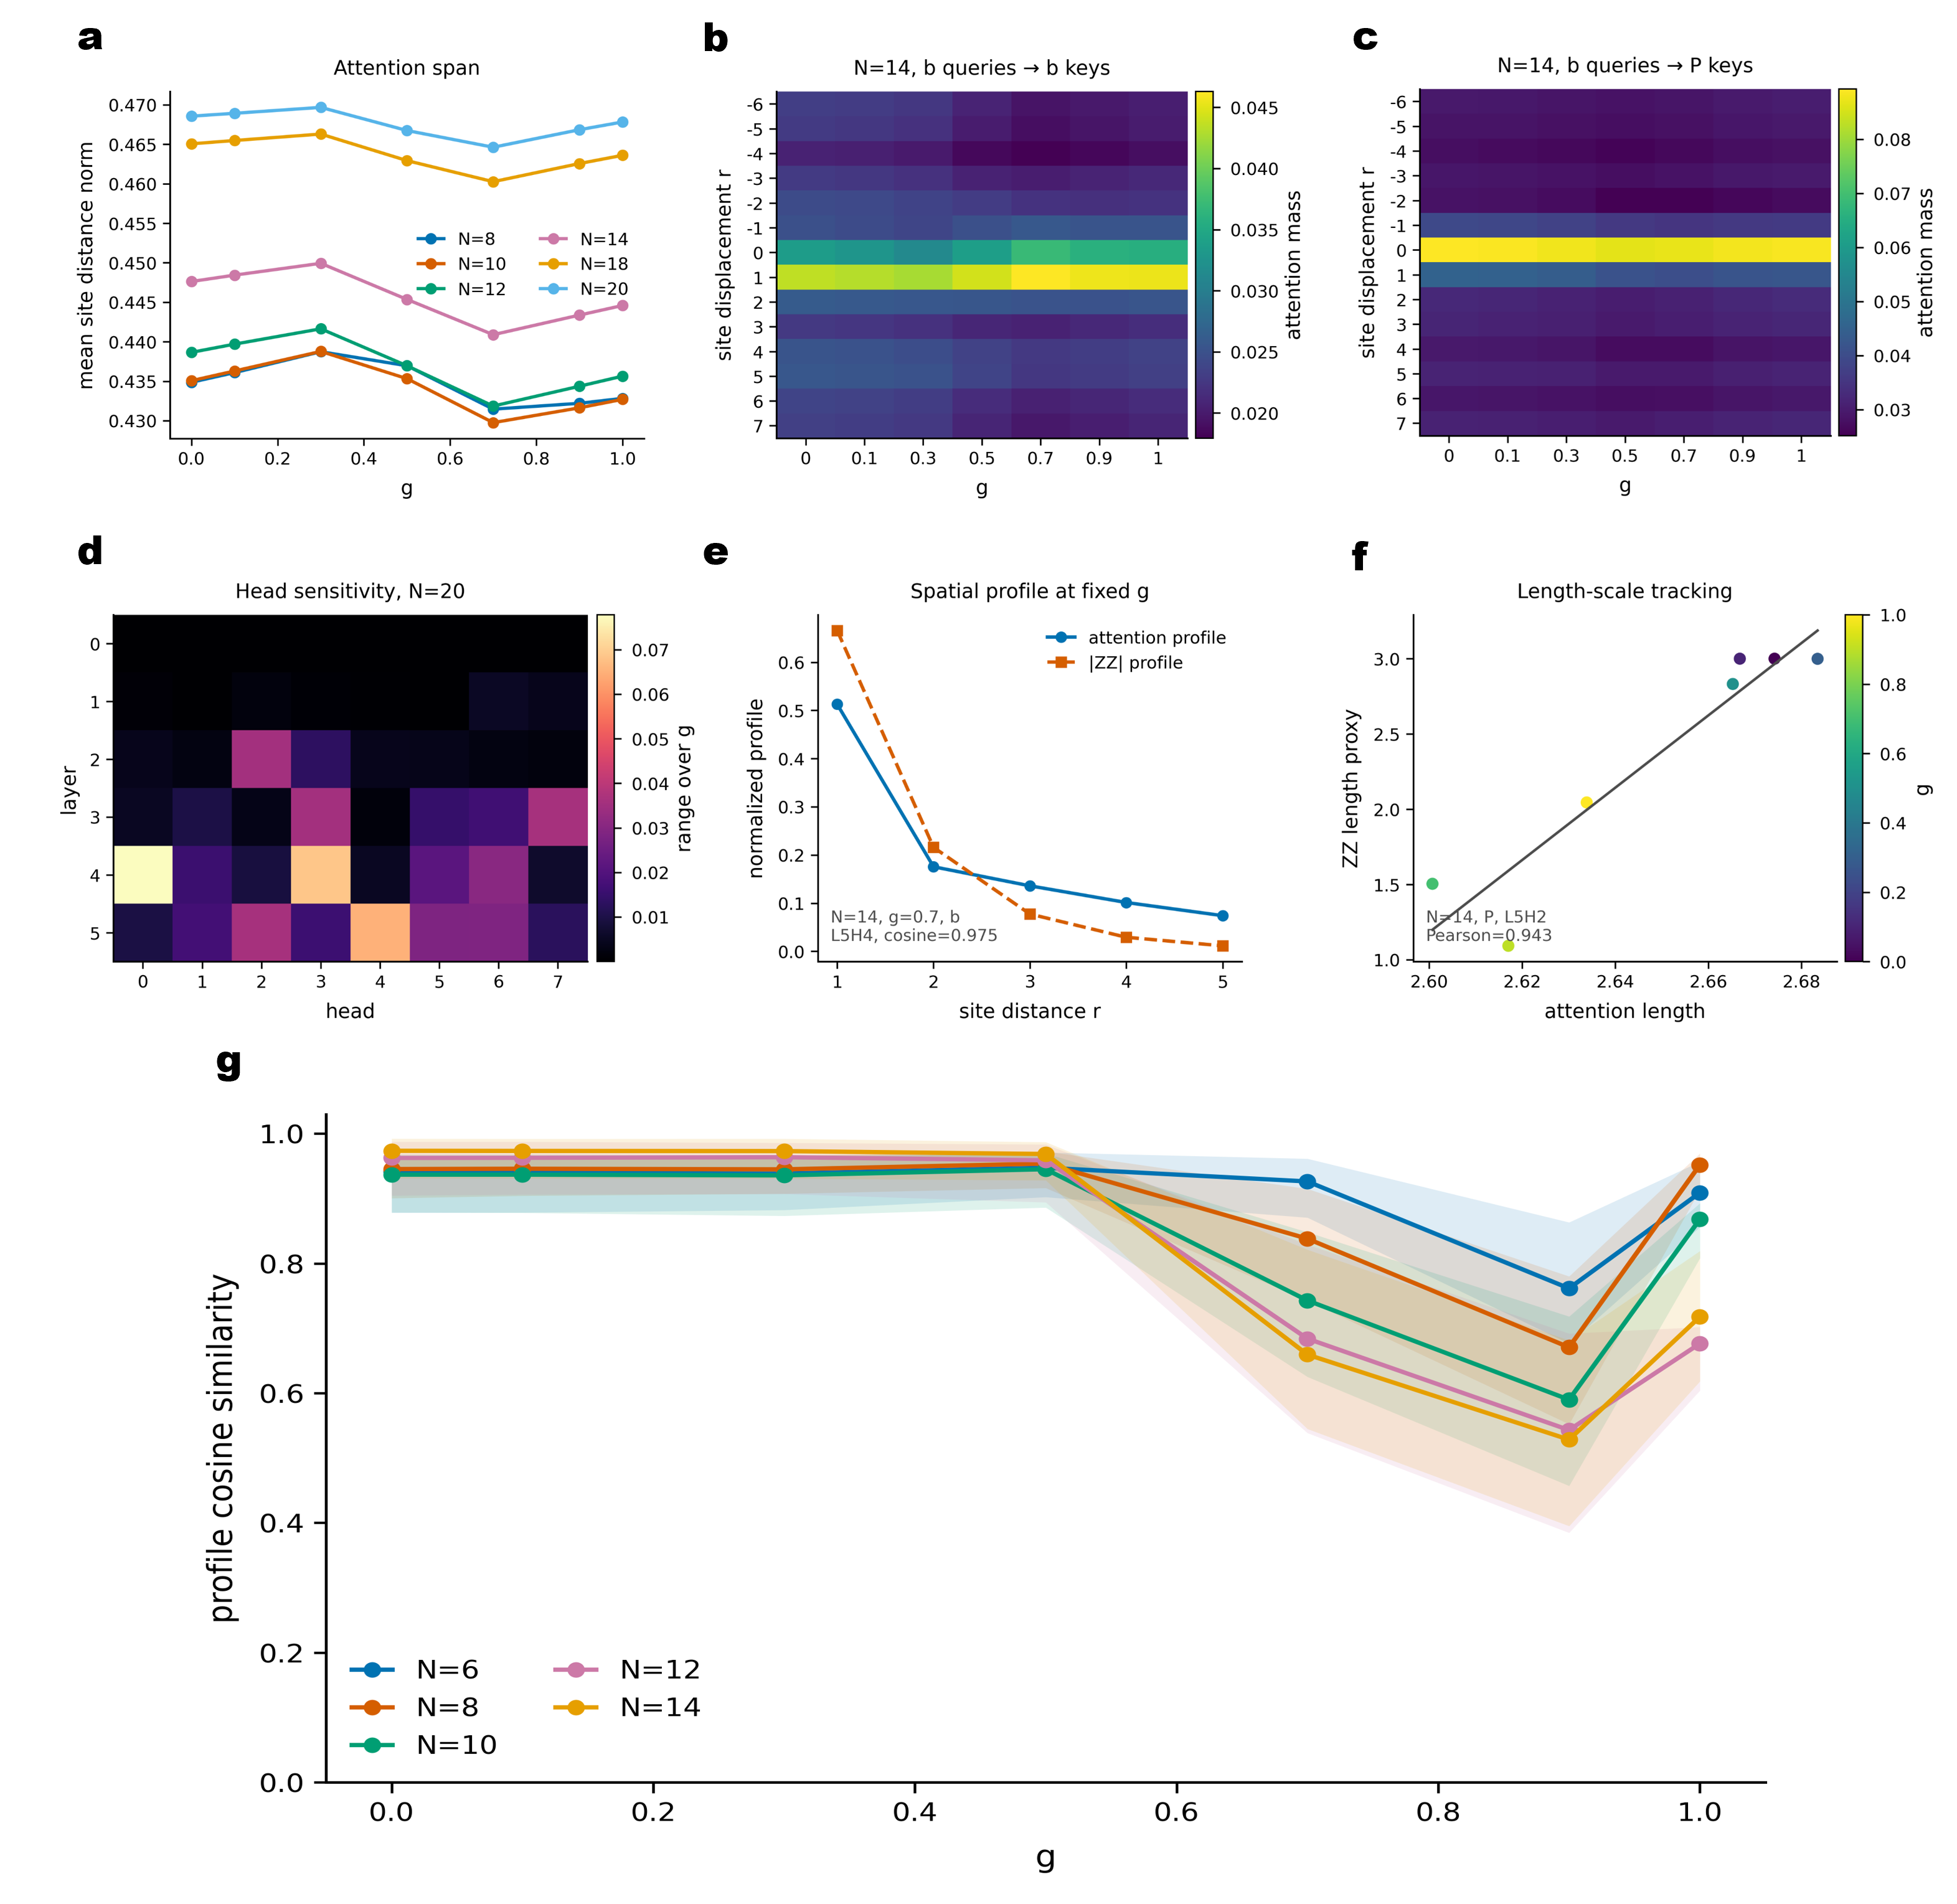
\includegraphics[width=0.98\textwidth]{fig/Figure4_all.png}
\caption{Attention mechanism analysis of Diffushadow.
(a) Normalized mean site distance as a function of the coupling parameter $g$. The metric measures the attention-weighted average lattice distance between masked measurement queries and site-indexed tokens, averaged over all heads and layers.
(b) Outcome-directed attention kernel $K_{bb}(r, g)$, showing the attention mass assigned from masked measurement outcomes to other measurement-outcome tokens as a function of lattice distance and coupling strength.
(c) Basis-directed attention kernel $K_{bP}(r, g)$, showing the attention mass assigned from masked measurement outcomes to measurement-basis tokens.
(d) Sensitivity of individual attention heads to the coupling parameter $g$, quantified by the variation of their attention-weighted mean site distances.
(e) Comparison between the absolute-distance attention kernel $K(\lvert r \rvert,g)$ of a representative specialized attention head and the corresponding exact correlation profile $\langle Z_i Z_{i+r} \rangle$.
(f) Relationship between the attention-weighted mean distance of the attention kernel and the correlation-weighted mean distance of the corresponding $ZZ$ correlation profile for a representative specialized head.
(g) Cosine similarity between the absolute-distance attention kernel and the corresponding $ZZ$ correlation profile as a function of coupling strength for different system sizes.
}\label{fig4}
\end{figure}


 
To further resolve the spatial structure of attention, we construct site-resolved attention kernels for measurement-basis tokens and measurement-outcome tokens. These kernels characterize how attention is distributed across different token types and lattice distances.
Specifically, the attention kernel $K(r, g)$ is defined as the average attention mass assigned to tokens located $r$ lattice sites away from a masked measurement query when the Hamiltonian parameter is $g$. 
% The kernel therefore characterizes how attention is distributed as a function of spatial separation and Hamiltonian parameter $g$. 
Depending on the token type of the attended keys, the kernel can be further decomposed into outcome-directed kernels $K_{bb}(r, g)$ and basis-directed kernels $K_{bP}(r, g)$, corresponding to attention allocated to measurement-outcome tokens and measurement-basis tokens, respectively. Figure \ref{fig4}b and c show how much attention a masked measurement token assigns to measurement-outcome tokens and measurement-basis tokens at different lattice distances, respectively.
Figure \ref{fig4}b reveals a pronounced concentration of attention at distances 0 and 1 across all coupling strengths. Beyond these local interactions, a clear phase-dependent pattern emerges. For $g<0.5$, substantial attention mass persists over a broad range of distances, leading to a relatively slow spatial decay and enhanced long-range information aggregation. In contrast, for $g>0.5$, attention becomes strongly localized, with distances 0 and 1 dominating the distribution and attention rapidly diminishing at larger separations. This behavior is consistent with the stronger long-range correlations present in the ferromagnetic phase of the transverse-field Ising model.
In Figure \ref{fig4}c, the attention mass is overwhelmingly concentrated at distance 0, far exceeding that at all other distances. This indicates that Diffushadow primarily relies on the measurement basis of the same site when predicting a masked measurement outcome, consistent with the fact that the local measurement basis provides the most direct information about the corresponding measurement result.


% For a masked measurement query token \(b_i\), we define a site-resolved attention kernel by aggregating attention over all key tokens of type
% \(\tau \in \{P,b\}\) at relative site displacement \(r\):
% \[
% K_{\tau}(r;g)
% =
% \left\langle
% \sum_{j}
% A(b_i,\tau_j)\,
% \mathbf{1}\!\left[j-i=r\right]
% \right\rangle_{i,\mathrm{prompts}},
% \qquad \tau \in \{P,b\}.
% \]
% where \(A_{\ell h}(q_i,\tau_j \mid g,N)\) is the attention weight in layer \(\ell\) and head \(h\) from the query token \(q_i=b_i\) to the key token \(\tau_j\), \(\mathcal{Q}\) denotes the set of masked measurement queries averaged over prompts and sites, and \(d(j,i)\) is the signed site displacement from query site \(i\) to key site \(j\) under periodic boundary conditions.

While the preceding analyses characterize the average attention behavior of the model, these aggregate statistics may conceal substantial heterogeneity across individual attention heads. We therefore examine the spatial attention patterns of individual heads. As shown in Figure \ref{fig4}d, we further probe the sensitivity of individual attention heads by quantifying how their attention patterns vary with the coupling parameter $g$. While attention heads in the first two layers remain largely invariant across different values of $g$, heads in deeper layers exhibit substantially stronger responses to changes in the physical regime. Such head-dependent behavior suggests a degree of functional specialization within the model, with different attention heads responding to different aspects of the underlying quantum correlations \cite{voita2019analyzing, michel2019sixteen}. This observation naturally raises the question of whether these specialized heads encode physically meaningful correlation structures. 

To investigate this possibility, we compare the spatial attention kernel of representative specialized heads with the exact correlation profile of the underlying quantum system. For this purpose, we introduce an absolute-distance attention kernel $K(\lvert r \rvert)$, obtained by combining attention weights associated with separations $+r$ and $-r$. As shown in Figure \ref{fig4}e, the attention kernel of a representative specialized head (L5H4) closely matches the corresponding correlation profile $\langle Z_i Z_{i+r}\rangle$ when $g=0.7$. The resulting cosine similarity reaches 0.975, indicating that, for this representative head and parameter setting, the spatial organization of attention is strongly aligned with the physical correlation structure encoded in the quantum state.
To further quantify the relationship between attention and physical correlations, we compare the characteristic spatial scales of the attention kernel and the correlation profile. Specifically, we compute the attention-weighted mean distance from the normalized kernel $K(\lvert r \rvert)$ and the correlation-weighted mean distance from the normalized correlation profile $\langle Z_i Z_{i+r}\rangle$. Figure \ref{fig4}f shows the resulting relationship for the specialized attention head L5H2 across different coupling parameters $g$. A strong linear correlation is observed ($\rho = 0.943$), suggesting that this attention head dynamically adjusts its effective receptive field according to the spatial extent of the physical correlations present in the quantum state.

While Figures \ref{fig4}e and \ref{fig4}f provide evidence from a representative specialized head, it remains important to assess whether the observed alignment persists across different physical regimes and system sizes. To characterize the model's behavior, we computed the cosine similarity between the attention kernel of each attention head and the corresponding correlation profile, averaging the results across different physical regimes and system sizes. As shown in Figure \ref{fig4}g, the similarity remains close to unity throughout the ordered regime $(g\leq 0.5)$ for all system sizes, indicating a high degree of similarity between the attention kernel and the corresponding correlation profile. Beyond the critical region, the similarity gradually decreases and reaches a minimum around $g \approx 0.9$, before increasing again as $g\to1.0$.
This decrease may be related to the weakening of $ZZ$ correlations in the paramagnetic regime. As $ZZ$ correlations become increasingly short-ranged, the learned attention pattern may no longer closely follow the corresponding correlation profile, resulting in a lower similarity.

In conclusion, these analyses suggest that Diffushadow develops a physically structured attention mechanism rather than merely learning sequence-level statistical patterns. The observed attention patterns show systematic correspondence with the spatial correlation structure of the transverse-field Ising model. This provides a mechanistic perspective on how the model captures many-body measurement distributions across different physical regimes and system sizes.

\section{Discussion}\label{sec12}

In this work, we introduced Diffushadow as a diffusion-based generative framework for scalable quantum measurement modeling. By learning from classical-shadow measurements of small quantum many-body systems, Diffushadow generates physically consistent measurement data beyond the original training sizes and enables downstream estimation of many-body observables. Across representative one-dimensional spin-chain Hamiltonians, the model reproduces key ground-state properties at both training and larger unseen system sizes, suggesting that the learned measurement structures can transfer across finite-size instances. Building on this capability, recursive scale extrapolation further expands the accessible system sizes and provides a route for inferring thermodynamic-limit properties from a limited set of exact small-system measurements.

We evaluated the applicability of Diffushadow on several representative one-dimensional spin-chain Hamiltonians, including the transverse-field Ising model, the frustrated $J_1$-$J_2$ model, and the ANNNI model. These systems cover both a canonical quantum phase-transition benchmark and spin-chain settings with competing interactions, providing a testbed beyond a single Hamiltonian. The same-size and cross-scale generation results show that Diffushadow can reproduce key physical observables not only within the training system size, but also at larger unseen sizes across these settings. In addition, finite-size extrapolation based on Diffushadow-generated measurements supports thermodynamic-limit inference for selected observables in these models.
% The transverse-field Ising model serves as the primary controlled benchmark for presenting the full pipeline, while the \(J_1\)-\(J_2\) and ANNNI results extend the analysis to frustrated and competing-interaction settings using model-specific observables. 
Thus, the present results support the transferability of Diffushadow across several one-dimensional spin-chain settings, while broader validation on more complex geometries and Hamiltonians remains an important direction for future work.
% We evaluated the applicability of Diffushadow on several representative one-dimensional spin-chain Hamiltonians, including the transverse-field Ising model, the frustrated \(J_1\)-\(J_2\) model, and the ANNNI model. The transverse-field Ising model serves as the primary controlled benchmark for presenting the full pipeline, from same-size measurement generation and cross-scale extrapolation to finite-size scaling and thermodynamic-limit inference. We further extended the analysis to the \(J_1\)-\(J_2\) and ANNNI models, which introduce frustration, competing interactions, dimerization physics, and modulated ordering tendencies. Using model-specific observables, including spin-dot correlations in the \(J_1\)-\(J_2\) model and structure factors in the ANNNI model, Diffushadow reproduces the main finite-size trends and supports selected thermodynamic-limit extrapolations beyond the transverse-field Ising setting. Thus, the present results support the transferability of Diffushadow across several one-dimensional spin-chain settings, while broader validation on more complex geometries, Hamiltonians, phases, and observables remains an important direction for future work.


The significance of this framework lies in connecting a generative modeling strategy with a concrete many-body physics objective. Classical-shadow tokenization allows Diffushadow to learn directly from experimentally accessible measurement records rather than from explicit wavefunction or density-matrix representations. Full-attention iterative denoising provides a flexible way to model globally correlated measurement configurations without imposing a predefined autoregressive ordering. Recursive scale extrapolation further turns this generative capability into a practical route for extending finite-size measurement data toward larger systems. In this sense, Diffushadow is not merely a model for producing additional samples, but a framework for using learned measurement distributions to support finite-size scaling and thermodynamic-limit inference.

The attention analysis provides additional insight into why Diffushadow can generalize across system sizes. In the transverse-field Ising setting, the spatial range of attention changes systematically across physical regimes, and selected attention heads develop kernels that closely follow exact spin-spin correlation profiles. These observations suggest that the model not only reproduces observable-level statistics, but also organizes information in a way that reflects the correlation structure of the underlying quantum state. Although attention patterns should not be interpreted as a complete explanation of the model's behavior \cite{jain2019attention}, they provide a mechanistic perspective on how full-attention denoising can capture transferable measurement structures across system sizes.

Several limitations remain. The present study focuses primarily on one-dimensional spin-chain Hamiltonians, and the mechanistic analyses are carried out in the transverse-field Ising setting. Extending Diffushadow to higher-dimensional systems, longer-range interactions, and more complex quantum phases will be important for assessing its broader applicability. In addition, the current experiments are based on numerically generated measurement data, whereas realistic quantum devices introduce sampling constraints, readout errors, and hardware-dependent noise that may affect the learned measurement distributions \cite{maciejewski2020mitigation, kim2022quantum}. Future work should therefore investigate Diffushadow on noisy experimental data, develop uncertainty-aware recursive extrapolation procedures, and examine how generated-measurement errors propagate into downstream physical estimates. Despite these open challenges, our results suggest that diffusion-based quantum measurement generation offers a promising framework for bridging accessible small-system measurements with larger-scale and thermodynamic-limit physics. By learning structured measurement distributions and enabling recursive extrapolation, Diffushadow provides a data-driven pathway that complements existing analytical and numerical approaches and may expand the practical reach of scalable inference in many-body quantum systems.




% \section{Conclusion}\label{sec13}

% Conclusions may be used to restate your hypothesis or research question, restate your major findings, explain the relevance and the added value of your work, highlight any limitations of your study, describe future directions for research and recommendations. 

% In some disciplines use of Discussion or 'Conclusion' is interchangeable. It is not mandatory to use both. Please refer to Journal-level guidance for any specific requirements. 



\section{Methods}\label{sec11}




\subsection{Quantum spin-chain Hamiltonians}

We consider three representative one-dimensional quantum spin-chain Hamiltonians to evaluate Diffushadow: the transverse-field Ising model \cite{pfeuty1970one}, the frustrated \(J_1\)-\(J_2\) model \cite{majumdar1969next, majumdar1969next2}, and the axial next-nearest-neighbor Ising (ANNNI) model \cite{selke1988annni}. Throughout this work, \(\sigma_i^\alpha\) with \(\alpha \in \{x,y,z\}\) denotes the Pauli operator acting on the \(i\)-th spin, and \(N\) denotes the number of spins. All three Hamiltonians are defined with periodic boundary conditions, such that
\begin{equation}
\sigma_{N+i}^{\alpha} = \sigma_i^{\alpha}.
\end{equation}

The first model is the one-dimensional transverse-field Ising model. In our numerical implementation, the Hamiltonian is parameterized by an interpolation parameter \(g\) between the Ising interaction and the transverse field,
\begin{equation}
H_{\mathrm{TFI}}(g)
=
-(1-g)\sum_{i=1}^{N}\sigma_i^z\sigma_{i+1}^z
-
g\sum_{i=1}^{N}\sigma_i^x .
\label{eq:tfi_hamiltonian}
\end{equation}
Here, \(g\) controls the relative strength of the transverse field. The Ising interaction dominates for small \(g\), whereas the transverse field dominates for large \(g\). In the thermodynamic limit, this parametrization gives the critical point at \(g_c=0.5\).

The second model is the frustrated \(J_1\)-\(J_2\) spin chain. We use the Pauli-matrix convention rather than the spin-operator convention \(S_i^\alpha=\sigma_i^\alpha/2\). The Hamiltonian is
\begin{equation}
H_{J_1\text{-}J_2}
=
J_1\sum_{i=1}^{N}
\left(
\sigma_i^x\sigma_{i+1}^x+
\sigma_i^y\sigma_{i+1}^y+
\sigma_i^z\sigma_{i+1}^z
\right)
+
J_2\sum_{i=1}^{N}
\left(
\sigma_i^x\sigma_{i+2}^x+
\sigma_i^y\sigma_{i+2}^y+
\sigma_i^z\sigma_{i+2}^z
\right).
\label{eq:j1j2_hamiltonian}
\end{equation}
Here, \(J_1\) and \(J_2\) denote the nearest-neighbor and next-nearest-neighbor exchange couplings, respectively. When \(J_1\) is fixed, we use
\begin{equation}
\alpha = \frac{J_2}{J_1},
\qquad
J_2 = \alpha J_1
\label{eq:j1j2_alpha}
\end{equation}
as the control parameter. When \(J_1=1\), the numerical value of \(\alpha\) is identical to that of \(J_2\). The next-nearest-neighbor coupling introduces competing interactions and frustration, making the \(J_1\)-\(J_2\) chain a useful benchmark beyond the transverse-field Ising model.

The third model is the transverse-field axial next-nearest-neighbor Ising model (ANNNI),
\begin{equation}
H_{\mathrm{ANNNI}}(g,\kappa)
=
-J_1\sum_{i=1}^{N}\sigma_i^z\sigma_{i+1}^z
+
\kappa J_1\sum_{i=1}^{N}\sigma_i^z\sigma_{i+2}^z
-
g\sum_{i=1}^{N}\sigma_i^x .
\label{eq:annni_hamiltonian}
\end{equation}
Here, \(J_1\) is the nearest-neighbor ferromagnetic Ising coupling, \(\kappa J_1\) is the competing next-nearest-neighbor Ising coupling, and \(g\) is the transverse-field strength. Equivalently,
\begin{equation}
J_2 = \kappa J_1 ,
\label{eq:annni_kappa}
\end{equation}
where \(\kappa\) controls the relative strength of the next-nearest-neighbor competing interaction. 
% In our experiments presented, \(J_1\) is fixed to \(1\), and the ANNNI model is evaluated by fixing \(\kappa\) and scanning the transverse field \(g\). 
This model provides an Ising-type spin-chain benchmark with competing interactions and richer finite-size behavior than the standard transverse-field Ising model.
In our experiments, \(J_1\) is fixed to \(1\), and the control parameters are \(J_2\) (i.e., \(\alpha\)) for the \(J_1\)-\(J_2\) model and \((g,\kappa)\) for the ANNNI model.


\subsection{Diffushadow architecture}
\label{sec:method_arch}


Diffushadow is implemented as a full-attention Transformer for discrete classical-shadow measurement sequences \cite{vaswani2017attention, huang2020predicting}. Each measurement snapshot is represented as an interleaved token sequence containing the Hamiltonian control parameter, the local measurement bases, and the corresponding measurement outcomes. For a system of \(N\) spins, the input sequence is written as
\begin{equation}
\mathbf{x}
=
[\boldsymbol{\lambda}, P_1, b_1, P_2, b_2, \ldots, P_N, b_N],
\end{equation}
where \(\boldsymbol{\lambda}\) denotes the scalar control parameter used in the corresponding experiment, \(P_i \in \{X,Y,Z\}\) is the Pauli measurement basis on site \(i\), and \(b_i\) is the measurement outcome. In the transverse-field Ising model and the ANNNI model with fixed \(\kappa\), \(\boldsymbol{\lambda}\) corresponds to the transverse-field parameter \(g\). In the \(J_1\)-\(J_2\) model, \(\boldsymbol{\lambda}\) corresponds to the coupling ratio \(\alpha=J_2/J_1\) (i.e., \(J_2\) when \(J_1=1\)).

The scalar control parameter is mapped to the model hidden dimension through a linear projection. This design avoids unnecessary dimensionality increase that could hinder learning and also reduces the overall complexity of the model. The measurement-basis tokens and measurement-outcome tokens are mapped through separate embedding layers, because they encode distinct types of information. For outcome tokens, an additional mask category is included to represent corrupted measurement outcomes during diffusion training. To distinguish the three types of tokens in the sequence, namely the control parameter, measurement bases, and measurement outcomes, we add a learnable type embedding to each token representation. The resulting embedded sequence is then passed to a stack of Transformer blocks.

Each Transformer block consists of multi-head full self-attention followed by a feed-forward network, with residual connections and layer normalization. Unlike causal autoregressive models, Diffushadow applies full attention over the entire sequence, allowing each measurement-outcome token to attend to the control parameter, all measurement bases, and all other available outcomes. This design avoids imposing a predefined left-to-right generation order and provides a flexible architecture for modeling globally correlated measurement configurations.
To encode positional information across variable system sizes, Diffushadow applies rotary positional embeddings (RoPE) to the query and key representations in each attention layer \cite{su2024roformer}. RoPE injects site-order information by applying position-dependent rotations to the query and key vectors, so that attention weights depend not only on token content but also on relative token positions. This provides a length-flexible positional encoding for classical-shadow sequences of different system sizes. The attention output is then projected back to the hidden dimension and passed through a feed-forward network with GELU activation.

The final output layer is a linear classifier applied only to the measurement-outcome positions. For each site \(i\), the model predicts a two-dimensional distribution over the binary measurement outcome,
\begin{equation}
p_\theta(b_i \mid \boldsymbol{\lambda}, \mathbf{P}, \mathbf{b}_t),
\end{equation}
where \(\mathbf{b}_t\) denotes the current partially masked measurement-outcome sequence. During training, only the masked positions contribute to the denoising loss. During generation, Diffushadow takes the current partially observed classical-shadow sequence as input and produces outcome predictions for all measurement-outcome positions. However, only the selected masked positions are updated at each denoising step. The same architecture is used for same-size generation, cross-scale generation, recursive scale extrapolation, and attention analysis.





\subsection{Training Diffushadow}
\label{sec:method_training}

Diffushadow is trained with a stochastic masking objective on classical-shadow measurement sequences. For each measurement snapshot, the conditioning information consists of the Hamiltonian control parameter \(\boldsymbol{\lambda}\) and the measurement-basis sequence \(\mathbf{P}\), while the measurement-outcome sequence is denoted by \(\mathbf{b}_0\). 
% Here, \(\boldsymbol{\lambda}\) represents the relevant model parameter, such as \(g\) for the transverse-field Ising model, \( J_2\) for the \(J_1\)-\(J_2\) model, and \((g,\kappa)\) for the ANNNI model.

During training, we corrupt only the measurement-outcome sequence \(\mathbf{b}_0\), while keeping \(\boldsymbol{\lambda}\) and \(\mathbf{P}\) unchanged. For each training sample, we first draw a masking probability
\begin{equation}
p_{\mathrm{mask}} \sim \mathcal{U}[\epsilon, 1],
\end{equation}
where \(\epsilon\) is a small positive hyperparameter that prevents the masking probability from being exactly zero. We then sample a binary mask sequence \(\mathbf{m}=(m_1,\ldots,m_N)\), where each mask variable is independently drawn as
\begin{equation}
m_i \sim \mathrm{Bernoulli}(p_{\mathrm{mask}}),
\end{equation}
and \(N\) is the number of spins for the corresponding sample. The corrupted outcome sequence \(\mathbf{b}_t\) is constructed by replacing masked positions with a special mask token \([\mathrm{MASK}]\):
\begin{equation}
\label{eq:mask_fun}
\mathbf{b}_t[i] =
\begin{cases}
[\mathrm{MASK}], & \text{if } m_i = 1, \\
\mathbf{b}_0[i], & \text{if } m_i = 0 .
\end{cases}
\end{equation}

For training on data spanning multiple system sizes, datasets from different system sizes are combined at the mini-batch level. Each mini-batch contains samples from only one fixed system size, so that all sequences within the batch have the same length. Mini-batches from different system sizes are then shuffled within each epoch and processed sequentially during training. In this way, Diffushadow is exposed to measurement data from multiple system sizes within the same training run, while each individual optimization step is performed on a batch with a consistent sequence length.

The training objective is to recover the original measurement outcomes at the masked positions, conditioned on the Hamiltonian parameter, the measurement bases, and the remaining unmasked outcomes. The denoising loss is defined as
\begin{equation}
\label{eq:loss_fun}
\mathcal{L}
=
-\mathbb{E}_{\boldsymbol{\lambda},\mathbf{P},\mathbf{b}_0,\mathbf{b}_t}
\left[
\sum_{i=1}^{N}
m_i
\log
p_{\theta}
\left(
\mathbf{b}_0[i]
\mid
\boldsymbol{\lambda},\mathbf{P},\mathbf{b}_t
\right)
\right],
\end{equation}
where \(p_{\theta}\) is the conditional distribution predicted by Diffushadow and \(\theta\) denotes the model parameters. Here, \(N\) denotes the system size of the current mini-batch. The factor \(m_i\) ensures that only masked positions contribute to the loss. Through this objective, Diffushadow learns to reconstruct missing measurement outcomes from the global measurement context, enabling iterative denoising during generation.



\subsection{Measurement generation and physical property estimation with Diffushadow}


To generate a classical-shadow measurement snapshot, Diffushadow starts from a fully masked measurement-outcome sequence. Given a Hamiltonian parameter \(\boldsymbol{\lambda}\) and a randomly sampled Pauli-basis sequence, the model iteratively predicts the corresponding measurement outcomes. At each denoising step, the model predicts probabilities for all masked positions. Instead of unmasking all positions simultaneously, we employ an adaptive strategy that selectively uncovers the most confident predictions in each iteration. Specifically, we compute the entropy of the model's output distribution as a measure of predictive uncertainty and unmask the positions with the lowest entropy (highest confidence). An ablation study of the decoding strategy is presented in Extended Data Table~\ref{tab:mse_table}, showing that iterative decoding with entropy-based position selection yields more accurate observable estimates than one-shot decoding or random position selection.






For each Hamiltonian parameter, Diffushadow generates \(M\) classical-shadow measurement snapshots \(\mathcal{D}=\{(\mathbf{P}_t,\mathbf{b}_t)\}_{t=1}^{M}\), where \(\mathbf{P}_t\) denotes the Pauli measurement-basis sequence and \(\mathbf{b}_t\) denotes the corresponding binary measurement-outcome sequence. The binary outcomes are mapped to Pauli eigenvalues as \(s_{t,i}=2b_{t,i}-1\). For the transverse-field Ising setting, we estimate longitudinal spin-spin correlations from the generated classical-shadow measurements. For uniformly sampled single-qubit Pauli measurements, the inverse measurement-channel factor gives the local estimator \(\widehat{Z}_{t,i}=3s_{t,i}\mathbf{1}[P_{t,i}=Z]\). The distance-\(r\) spin-spin correlation is then estimated under periodic boundary conditions as
\begin{equation}
\widehat{C}_{ZZ}(r)
=
\frac{1}{MN}
\sum_{t=1}^{M}
\sum_{i=1}^{N}
\widehat{Z}_{t,i}
\widehat{Z}_{t,i+r},
\qquad
\end{equation}
where the site index $i+r$ is understood modulo $N$.

For the \(J_1\)-\(J_2\) model, we estimate spin-dot correlations from the same classical-shadow snapshots. For each Pauli component \(\alpha\in\{x,y,z\}\), we define the local estimator
\[
\widehat{\sigma}^{\alpha}_{t,i}
=
3s_{t,i}\mathbf{1}[P_{t,i}=\alpha].
\]
The component-resolved spin correlation is estimated as
\begin{equation}
\widehat{C}_{\alpha\alpha}(r)
=
\frac{1}{MN}
\sum_{t=1}^{M}
\sum_{i=1}^{N}
\widehat{\sigma}^{\alpha}_{t,i}
\widehat{\sigma}^{\alpha}_{t,i+r},
\end{equation}
where \(i+r\) is again understood modulo \(N\). The spin-dot correlation is then computed as
\begin{equation}
\widehat{C}_{\mathrm{spin}}(r)
=
\widehat{C}_{xx}(r)
+
\widehat{C}_{yy}(r)
+
\widehat{C}_{zz}(r),
\end{equation}
corresponding to
\(\langle\boldsymbol{\sigma}_i\cdot\boldsymbol{\sigma}_{i+r}\rangle\).
In the finite-size generation tests, we evaluate \(r=1,2,3\), while the thermodynamic-limit analysis focuses on \(r=1,2\), which directly correspond to the nearest- and next-nearest-neighbor exchange terms in the \(J_1\)-\(J_2\) Hamiltonian.

For the ANNNI model, we estimate the longitudinal structure factor from the \(ZZ\) correlations. Using the translationally averaged correlation \(\widehat{C}_{ZZ}(r)\), the structure factor at momentum \(q\) is computed as
\begin{equation}
\widehat{S}_{Z}(q)
=
\sum_{r=0}^{N-1}
e^{iqr}
\widehat{C}_{ZZ}(r).
\end{equation}
In the main text, we evaluate \(q=\pi\) and \(q=\pi/2\), which probe staggered and period-four modulated ordering components, respectively.



To reduce estimator variance, we use a median-of-means aggregation. The generated snapshots are divided into \(K\) subsets, each observable estimator is computed independently on each subset, and the final estimate is taken as
\begin{equation}
\widehat{C}^{\mathrm{MoM}}_{ZZ}(r)
=
\operatorname{median}_{k=1,\ldots,K}
\widehat{C}^{(k)}_{ZZ}(r).
\end{equation}
In our implementation, we set \(K=10\). The same estimation procedure is applied to both exact and Diffushadow-generated measurement snapshots when comparing physical observables.



\subsection{Attention analysis}
\label{sec:method_attention}

To investigate the internal spatial organization learned by Diffushadow, we analyze the attention maps produced by trained Diffushadow. The input sequence consists of a Hamiltonian-parameter token, local measurement-basis tokens \(P_i\), and measurement-outcome tokens \(b_i\). We focus on masked measurement-outcome tokens as query tokens, because these are the positions reconstructed during the denoising process.

Let \(A^{(\ell,h)}_{qk}\) denote the attention weight from query token \(q\) to key token \(k\) in layer \(\ell\) and head \(h\). For each site-indexed token, we assign a lattice site index \(s(k)\). The set of site-indexed tokens \(\mathcal{S}\) includes both measurement-basis tokens \(P_i\) and measurement-outcome tokens \(b_i\). For a masked outcome query token \(q\) located at site \(s(q)\), we define its attention-weighted site distance as
\begin{equation}
D^{(\ell,h)}(q)
=
\sum_{k\in\mathcal{S}}
A^{(\ell,h)}_{qk}
\,d_N\!\left(s(q),s(k)\right),
\end{equation}
where \(d_N(\cdot,\cdot)\) denotes the periodic lattice distance between two sites. We average this quantity over masked query positions and, unless otherwise specified, over all layers and heads. To compare systems of different sizes, the resulting mean site distance is normalized by the maximum possible periodic lattice distance.

To resolve how attention is distributed across token types and spatial separations, we construct site-resolved attention kernels. Here, \(r\) denotes the signed lattice displacement between the query site and the key site, evaluated under periodic boundary conditions. For a masked outcome query token \(b_i\), the outcome-directed and basis-directed kernels are defined as functions of \(r=j-i\):
\begin{equation}
K_{bb}^{(\ell,h)}(r)
=
\left\langle
\sum_{j:\,j-i=r}
A^{(\ell,h)}_{b_i,b_j}
\right\rangle_i,
\qquad
K_{bP}^{(\ell,h)}(r)
=
\left\langle
\sum_{j:\,j-i=r}
A^{(\ell,h)}_{b_i,P_j}
\right\rangle_i ,
\end{equation}
where \(\langle\cdot\rangle_i\) denotes averaging over query sites. These kernels quantify how much attention a masked measurement outcome assigns to measurement-outcome tokens and measurement-basis tokens at different lattice separations. For visualizing the average model behavior, the kernels are averaged over layers, heads, samples, and query sites. For head-level analysis, they are kept separately for each layer and head.

We further quantify the sensitivity of individual attention heads to changes in the Hamiltonian parameter. For each layer and head, we compute the variation of its attention-weighted mean site distance across different values of \(g\):
\begin{equation}
\Delta D^{(\ell,h)}
=
\max_g \overline{D}^{(\ell,h)}(g)
-
\min_g \overline{D}^{(\ell,h)}(g),
\end{equation}
where \(\overline{D}^{(\ell,h)}(g)\) denotes the mean site distance of head \(h\) in layer \(\ell\) at coupling strength \(g\). This quantity measures how strongly the spatial attention pattern of each head changes across physical regimes.

To compare learned attention structures with physical correlation structures, we use the outcome-directed attention kernel \(K_{bb}\), which directly describes attention between measurement-outcome tokens. Unless otherwise specified, all comparisons with \(ZZ\) correlations are performed using this kernel. We first construct an absolute-distance attention kernel by aggregating opposite displacements, \(K_{bb}(|r|)=K_{bb}(r)+K_{bb}(-r)\) for \(r>0\), with \(K_{bb}(|0|)=K_{bb}(0)\). This profile is compared with the absolute two-point correlation profile \(C_{ZZ}(r)=|\langle Z_iZ_{i+r}\rangle|\). Both profiles are normalized over the distances used for comparison, giving \(\widetilde{K}_{bb}(|r|)\) and \(\widetilde{C}_{ZZ}(r)\). Their similarity is measured by
\begin{equation}
S_{\mathrm{cos}}
=
\frac{
\sum_r
\widetilde{K}_{bb}(|r|)
\widetilde{C}_{ZZ}(r)
}{
\sqrt{
\sum_r
\widetilde{K}_{bb}(|r|)^2
}
\sqrt{
\sum_r
\widetilde{C}_{ZZ}(r)^2
}
}.
\end{equation}
This metric measures the degree to which the spatial shape of the learned attention kernel aligns with the corresponding physical correlation profile.

Finally, we compare the characteristic spatial extent of the learned attention kernel with that of the exact \(ZZ\) correlation profile. We compute first-moment measures
\begin{equation}
\ell_{\mathrm{attn}}
=
\sum_r r\,\widetilde{K}_{bb}(|r|),
\qquad
\ell_{ZZ}
=
\sum_r r\,\widetilde{C}_{ZZ}(r).
\end{equation}
These quantities are not intended to represent conventional correlation lengths. Instead, they provide comparable measures of the spatial extent of the attention and correlation profiles, allowing us to assess whether the learned attention pattern tracks the characteristic spatial range of the underlying quantum correlations.






% Topical subheadings are allowed. Authors must ensure that their Methods section includes adequate experimental and characterization data necessary for others in the field to reproduce their work. Authors are encouraged to include RIIDs where appropriate. 

% \textbf{Ethical approval declarations} (only required where applicable) Any article reporting experiment/s carried out on (i)~live vertebrate (or higher invertebrates), (ii)~humans or (iii)~human samples must include an unambiguous statement within the methods section that meets the following requirements: 

% \begin{enumerate}[1.]
% \item Approval: a statement which confirms that all experimental protocols were approved by a named institutional and/or licensing committee. Please identify the approving body in the methods section

% \item Accordance: a statement explicitly saying that the methods were carried out in accordance with the relevant guidelines and regulations

% \item Informed consent (for experiments involving humans or human tissue samples): include a statement confirming that informed consent was obtained from all participants and/or their legal guardian/s
% \end{enumerate}

% If your manuscript includes potentially identifying patient/participant information, or if it describes human transplantation research, or if it reports results of a clinical trial then  additional information will be required. Please visit (\url{https://www.nature.com/nature-research/editorial-policies}) for Nature Portfolio journals, (\url{https://www.springer.com/gp/authors-editors/journal-author/journal-author-helpdesk/publishing-ethics/14214}) for Springer Nature journals, or (\url{https://www.biomedcentral.com/getpublished/editorial-policies\#ethics+and+consent}) for BMC.


\backmatter

\bmhead{Supplementary information}

If your article has accompanying supplementary file/s please state so here. 

Authors reporting data from electrophoretic gels and blots should supply the full unprocessed scans for key as part of their Supplementary information. This may be requested by the editorial team/s if it is missing.

Please refer to Journal-level guidance for any specific requirements.

\bmhead{Acknowledgements}

Acknowledgements are not compulsory. Where included they should be brief. Grant or contribution numbers may be acknowledged.

Please refer to Journal-level guidance for any specific requirements.

\section*{Declarations}

Some journals require declarations to be submitted in a standardised format. Please check the Instructions for Authors of the journal to which you are submitting to see if you need to complete this section. If yes, your manuscript must contain the following sections under the heading `Declarations':

\begin{itemize}
\item Funding
\item Conflict of interest/Competing interests (check journal-specific guidelines for which heading to use)
\item Ethics approval and consent to participate
\item Consent for publication
\item Data availability 
\item Materials availability
\item Code availability 
\item Author contribution
\end{itemize}

\noindent
If any of the sections are not relevant to your manuscript, please include the heading and write `Not applicable' for that section. 

%%===================================================%%
%% For presentation purpose, we have included        %%
%% \bigskip command. Please ignore this.             %%
%%===================================================%%
% \bigskip
% \begin{flushleft}%
% Editorial Policies for:

% \bigskip\noindent
% Springer journals and proceedings: \url{https://www.springer.com/gp/editorial-policies}

% \bigskip\noindent
% Nature Portfolio journals: \url{https://www.nature.com/nature-research/editorial-policies}

% \bigskip\noindent
% \textit{Scientific Reports}: \url{https://www.nature.com/srep/journal-policies/editorial-policies}

% \bigskip\noindent
% BMC journals: \url{https://www.biomedcentral.com/getpublished/editorial-policies}
% \end{flushleft}

% \begin{appendices}

% \section{Section title of first appendix}\label{secA1}

% An appendix contains supplementary information that is not an essential part of the text itself but which may be helpful in providing a more comprehensive understanding of the research problem or it is information that is too cumbersome to be included in the body of the paper.

% %%=============================================%%
% %% For submissions to Nature Portfolio Journals %%
% %% please use the heading ``Extended Data''.   %%
% %%=============================================%%
\setcounter{figure}{0}
\setcounter{table}{0}
\renewcommand{\figurename}{Extended Data Fig.}
\renewcommand{\tablename}{Extended Data Table}


\begin{table*}[htbp]
\centering
\setlength{\tabcolsep}{8pt}
% \small
\caption{MSE of Model Predictions (Diffushadow, ShadowGPT) and Exact Values for the ground-state energy and three spin-spin correlations. ShGPT denotes ShadowGPT, Diffu-rdm denotes Diffushadow with randomly selected decoding positions, Diffu-s1 denotes Diffushadow decoding in one step, Diffu denotes the full Diffushadow.}
\label{tab:mse_table}
\begin{tabular}{llcccc}
\hline
 &Model & $E_0$ & $\langle Z_iZ_{i+1}\rangle$ & $\langle Z_iZ_{i+3}\rangle$ & $\langle Z_iZ_{i+5}\rangle$\\
\hline
\multirow{4}{*}{$g=0.1$} 
& ShGPT      & $3.63{\times}10^{-4}$ & $2.64{\times}10^{-8}$ & $6.51{\times}10^{-6}$ & $\mathbf{9.00{\times}10^{-6}}$\\
& Diffu-rdm & $2.34{\times}10^{-3}$ & $2.63{\times}10^{-8}$ & $9.00{\times}10^{-6}$ & $1.30{\times}10^{-5}$\\
& Diffu-s1  & $7.99{\times}10^{1}$ & $1.01{\times}10^{0}$ & $1.00{\times}10^{0}$ & $1.02{\times}10^{0}$\\
& \textbf{Diffu}    & $\underline{\mathbf{2.77{\times}10^{-4}}}$ & $\underline{\mathbf{2.47{\times}10^{-8}}}$ & $\underline{\mathbf{1.44{\times}10^{-6}}}$ & $1.10{\times}10^{-5}$\\
\hline
\multirow{4}{*}{$g=0.5$} 
& ShGPT      & $1.35{\times}10^{-2}$ & $6.30{\times}10^{-4}$ & $1.09{\times}10^{-3}$ & $4.80{\times}10^{-4}$\\
& Diffu-rdm & $7.59{\times}10^{-3}$ & $1.97{\times}10^{-4}$ & $9.42{\times}10^{-4}$ & $6.46{\times}10^{-4}$\\
& Diffu-s1  & $1.00{\times}10^{1}$ & $4.10{\times}10^{-1}$ & $2.58{\times}10^{-1}$ & $2.44{\times}10^{-1}$\\
& \textbf{Diffu}    & $\underline{\mathbf{7.13{\times}10^{-3}}}$ & $\underline{\mathbf{1.61{\times}10^{-4}}}$ & $\underline{\mathbf{4.00{\times}10^{-4}}}$ & $\underline{\mathbf{2.12{\times}10^{-4}}}$\\
\hline
\multirow{4}{*}{$g=0.9$} 
& ShGPT      & $6.79{\times}10^{-4}$ & $6.27{\times}10^{-4}$ & $2.28{\times}10^{-5}$ & $5.20{\times}10^{-5}$\\
& Diffu-rdm & $5.05{\times}10^{-4}$ & $1.26{\times}10^{-4}$ & $1.07{\times}10^{-4}$ & $1.10{\times}10^{-4}$\\
& Diffu-s1  & $1.47{\times}10^{-3}$ & $4.11{\times}10^{-3}$ & $2.58{\times}10^{-5}$ & $9.82{\times}10^{-5}$\\
& \textbf{Diffu}    & $\underline{\mathbf{4.98{\times}10^{-4}}}$ & $\underline{\mathbf{5.39{\times}10^{-5}}}$ & $\underline{\mathbf{5.15{\times}10^{-6}}}$ & $\underline{\mathbf{3.70{\times}10^{-7}}}$\\
\hline
\end{tabular}
\end{table*}



\begin{figure}[htbp]
  \centering
  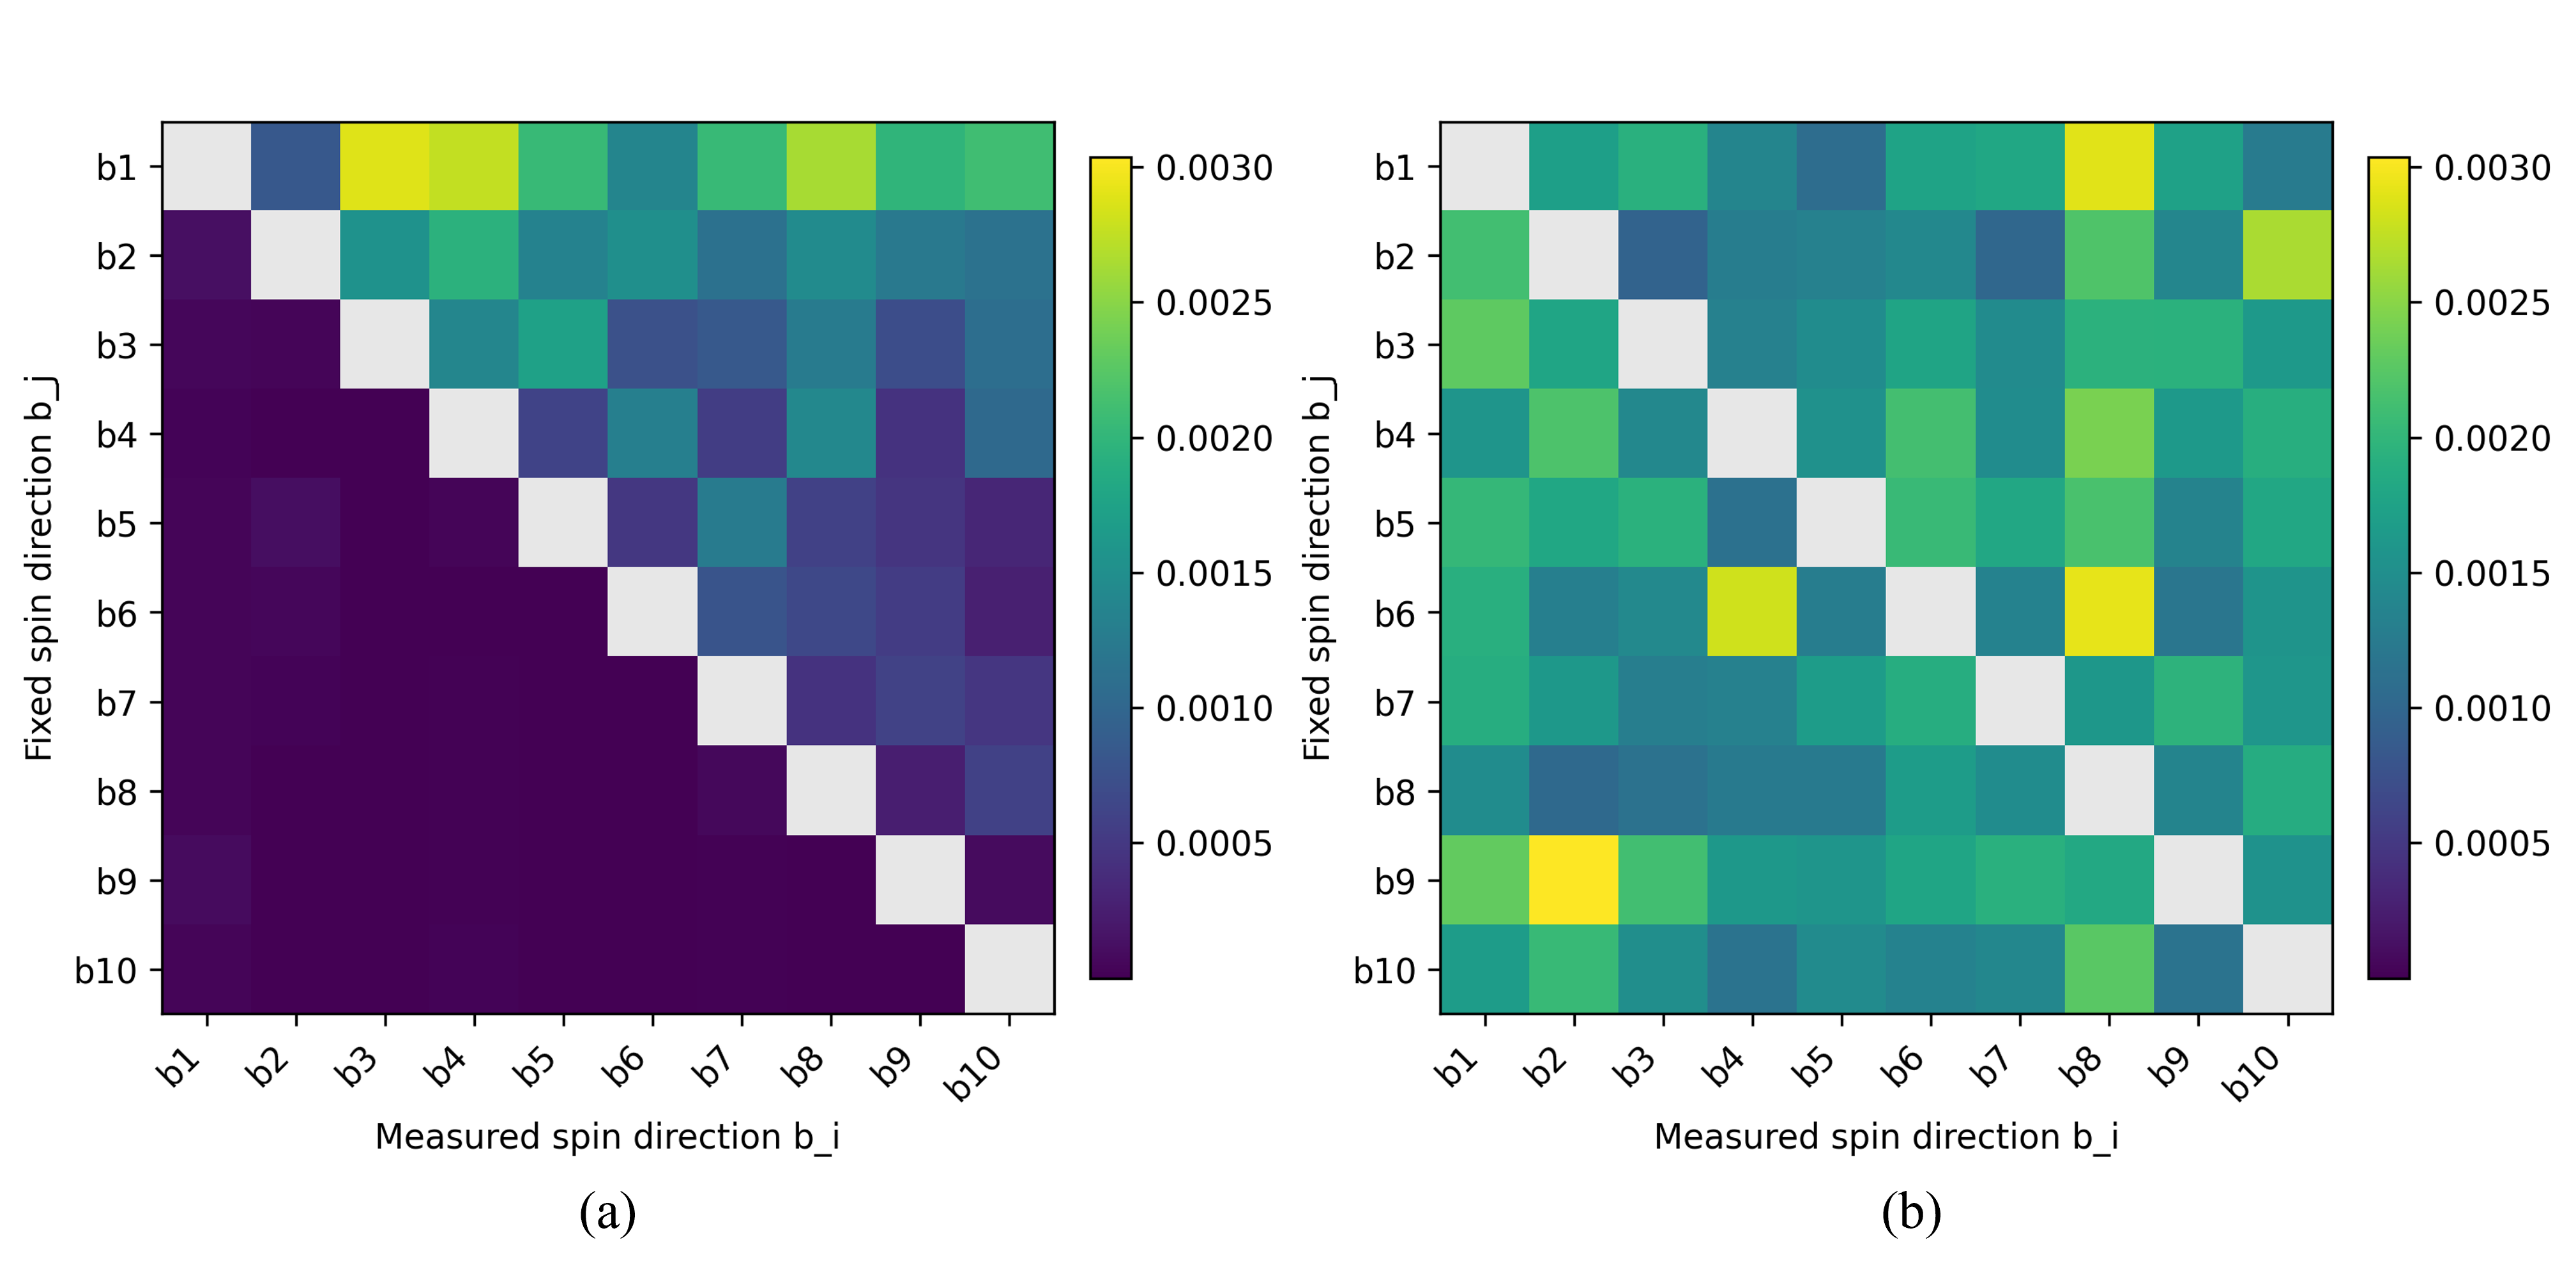
\includegraphics[width=0.98\textwidth]{fig/kl_control_to_experiment_heatmaps2.png}
  \caption{KL divergence of the predicted distributions of the remaining qubits after fixing the measurement outcome of a selected qubit. (a) The result of Diffushadow with causal attention. (b) The result of Diffushadow.
  Full attention allows the perturbation to influence both earlier and later sequence positions, whereas causal attention primarily propagates the perturbation to later positions.}
  \label{fig:kl_divergence_attention}    
\end{figure}



% \begin{figure}[htbp]
%   \centering
%   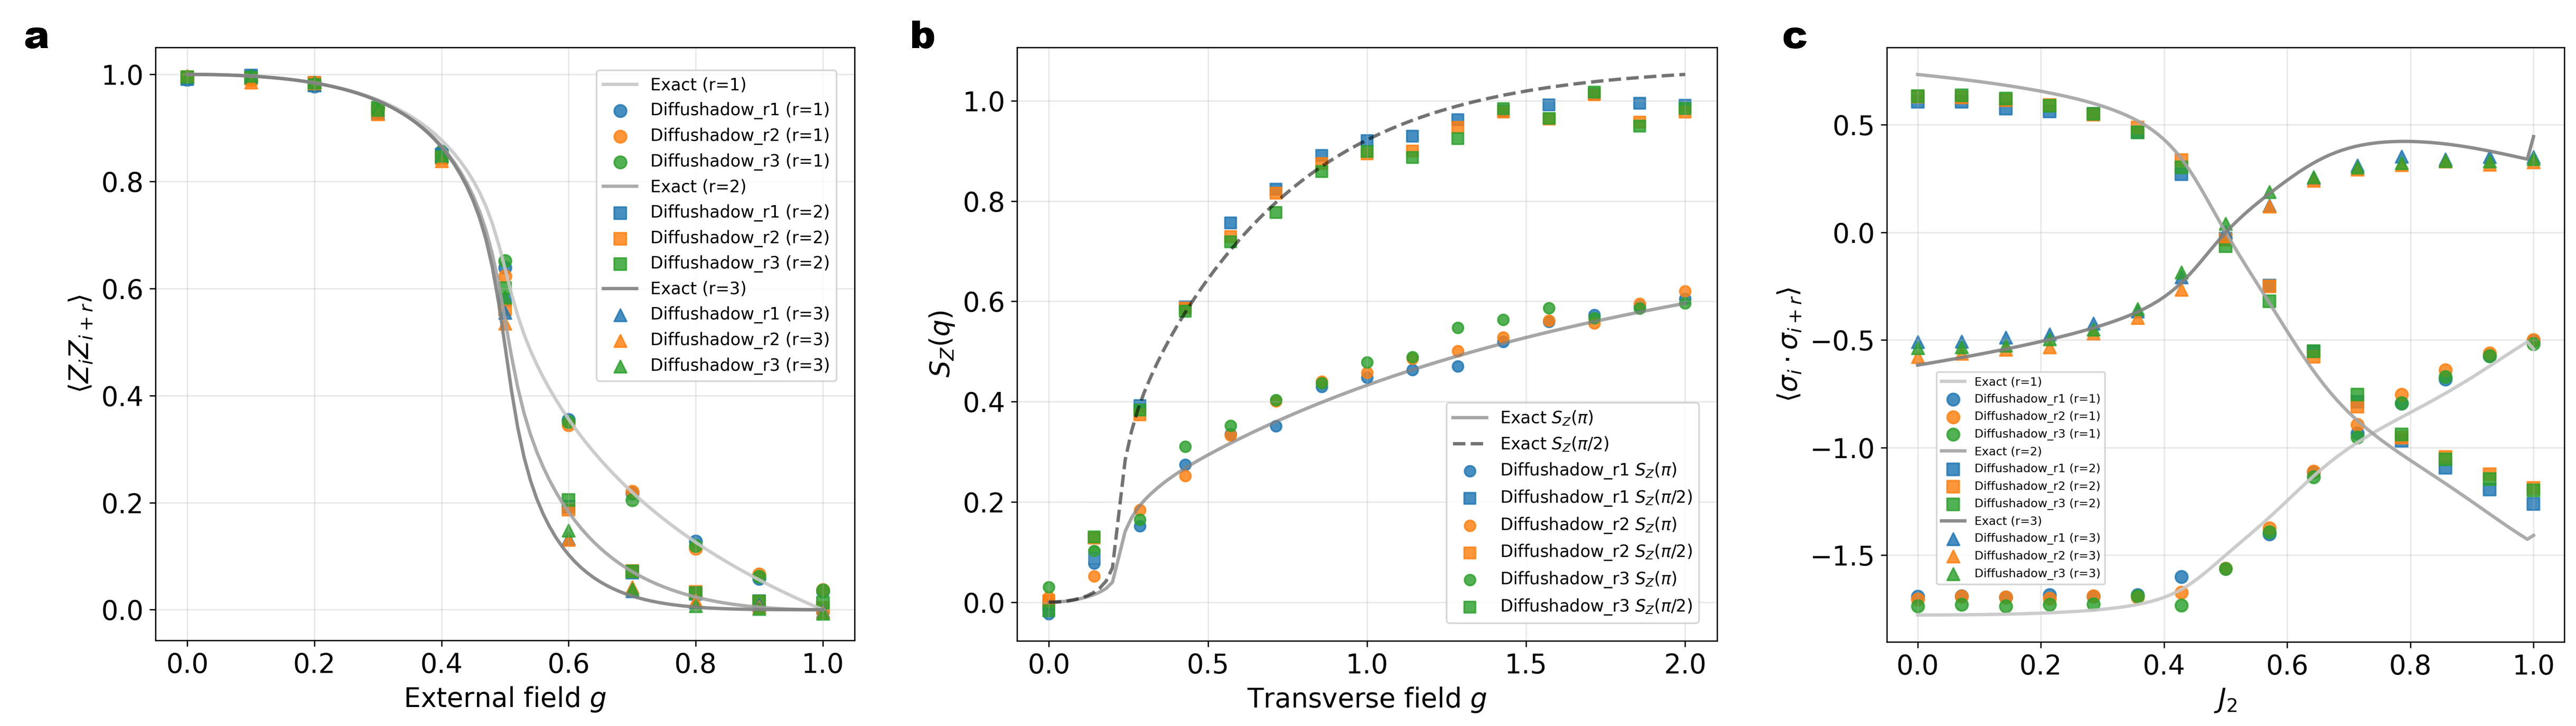
\includegraphics[width=0.98\textwidth]{fig/Figure_stability_all.png}
%   \caption{KL divergence of the predicted distributions of the remaining qubits after fixing the measurement outcome of a selected qubit. (a) The result of Diffushadow with causal attention. (b) The result of Diffushadow.
%   Full attention allows the perturbation to influence both earlier and later sequence positions, whereas causal attention primarily propagates the perturbation to later positions.}
%   \label{fig:kl_divergence_attention}    
% \end{figure}

% %%=============================================================%%
% %% Sample for another appendix section			       %%
% %%=============================================================%%

% %% \section{Example of another appendix section}\label{secA2}%
% %% Appendices may be used for helpful, supporting or essential material that would otherwise 
% %% clutter, break up or be distracting to the text. Appendices can consist of sections, figures, 
% %% tables and equations etc.

% \end{appendices}

%%===========================================================================================%%
%% If you are submitting to one of the Nature Portfolio journals, using the eJP submission   %%
%% system, please include the references within the manuscript file itself. You may do this  %%
%% by copying the reference list from your .bbl file, paste it into the main manuscript .tex %%
%% file, and delete the associated \verb+\bibliography+ commands.                            %%
%%===========================================================================================%%

\bibliography{sn-bibliography}% common bib file
%% if required, the content of .bbl file can be included here once bbl is generated
%%\input sn-article.bbl

\end{document}
